\documentclass[a4paper]{extarticle}

\usepackage[margin=1cm]{geometry}
\usepackage{multicol}
\setlength\columnsep{20pt}
\setlength{\columnseprule}{0.1pt} 

\setlength\parindent{0pt}

\usepackage[ngerman]{babel} % Silbentrennung
\usepackage[utf8]{inputenc} % Umlaute

\usepackage{mathpazo}
\usepackage{microtype}

\usepackage{picture}
\usepackage{graphicx}

\usepackage{float}

\usepackage{mathtools}
\usepackage{amsmath}
\usepackage{amssymb}

% allow page break in align* environment
\allowdisplaybreaks

\usepackage{booktabs}

\usepackage{enumitem}
\setlist{noitemsep,topsep=3pt,parsep=3pt,partopsep=3pt,leftmargin=15pt}
\renewcommand\labelitemi{{\boldmath$\cdot$}}
\newcommand{\listarrow}{
\smash{\scalebox{1.5}[1.75]{\rotatebox[origin=c]{180}{$\Lsh$}}}
}

\usepackage{comment}

\usepackage{cancel}

% COLORS
\usepackage{color}
\definecolor{defcolor}{rgb}{0.75, 1, 0.75}
\definecolor{thmcolor}{rgb}{1, 0.75, 0.75}
\definecolor{titlecolor}{rgb}{0,0,0}
%\definecolor{defcolor}{rgb}{0.64, 1, 0.29}
%\definecolor{thmcolor}{rgb}{1, 0.43, 0.39}
%\definecolor{titlecolor}{rgb}{0,0,0}
%\definecolor{defcolor}{rgb}{0.25, 0.45, 0.12}
%\definecolor{thmcolor}{rgb}{0.66, 0.32, 0.32}


\usepackage{xifthen}
% removed outside, to avoid long lines
\newcommand{\emptyarg}[1][]{\ifthenelse{\isempty{#1}}{}{\ (#1)}}

\newcommand{\Def}[1][]{\colorbox{defcolor}{\color{titlecolor}{\textbf{D.\emptyarg[#1]}}}\kern+0.3ex}
\newcommand{\Thm}[1][]{\colorbox{thmcolor}{\color{titlecolor}{\textbf{T.\emptyarg[#1]}}}\kern+0.3ex}
\newcommand{\Lem}[1][]{\colorbox{thmcolor}{\color{titlecolor}{\textbf{L.\emptyarg[#1]}}}\kern+0.3ex}
\newcommand{\Cor}[1][]{\colorbox{thmcolor}{\color{titlecolor}{\textbf{C.\emptyarg[#1]}}}\kern+0.3ex}
\newcommand{\Fact}{\textbf{Fact.}\ }
\newcommand{\Proof}{\textbf{Proof.}\ }
\newcommand{\Com}{\textbf{Com.}\ }
\newcommand{\Ex}{\textbf{Example:}\ }
\newcommand{\Trick}{\textbf{Trick:}\ }


% NUMBER SYSTEMS
\newcommand{\N}{\mathbb{N}}
\newcommand{\Z}{\mathbb{Z}}
\newcommand{\Q}{\mathbb{Q}}
\newcommand{\R}{\mathbb{R}}
\newcommand{\C}{\mathbb{C}}

% CALLICGRAPHIC SHORTCUTS
\newcommand{\cA}{\mathcal{A}}
\newcommand{\cS}{\mathcal{S}}
\newcommand{\cP}{\mathcal{P}}
\newcommand{\cU}{\mathcal{U}}
\newcommand{\cK}{\mathcal{K}}

% todo: symbol
\DeclareMathOperator{\id}{\text{id}}

% RELATIONS
\newcommand{\relid}{\mathrel{\id}}
\newcommand{\relrho}{\mathrel{\rho}}
\newcommand{\relsigma}{\mathrel{\sigma}}
\newcommand{\reltheta}{\mathrel{\theta}}
\newcommand{\relsim}{\mathrel{\sim}}
\newcommand{\relf}{\mathrel{f}}
\newcommand{\invrelid}{\mathrel{\widehat{\id}}}
\newcommand{\invrelrho}{\mathrel{\widehat{\rho}}}
\newcommand{\invrelsigma}{\mathrel{\widehat{\sigma}}}
\newcommand{\invreltheta}{\mathrel{\widehat{\theta}}}
\newcommand{\invrelsim}{\mathrel{\widehat{\sim}}}
\newcommand{\invrelf}{\mathrel{\widehat{f}}}

% BRACES
\newcommand{\alg}[1]{\langle #1 \rangle}
\newcommand{\card}[1]{\lvert #1 \rvert}
\newcommand{\abs}[1]{\lvert #1 \rvert}
\newcommand{\ceil}[1]{\lceil #1 \rceil}
\newcommand{\floor}[1]{\lfloor #1 \rfloor}

% OPERATORS
\DeclareMathOperator{\lcm}{lcm}
\DeclareMathOperator{\glb}{glb}
\DeclareMathOperator{\lub}{lub}
\DeclareMathOperator{\im}{im}
\DeclareMathOperator{\ord}{ord}

% LOGIC
\newcommand{\derives}{\vdash}

\newcommand{\rtop}{\reflectbox{\rotatebox[origin=c]{180}{$\top$}}}

% SEPARATOR
\newcommand{\sep}{\vspace{5pt}\noindent\hrule\vspace{5pt}}

% todo COMMAND
\newcommand{\todo}[1]{\textcolor{red}{TODO: #1}}

\begin{document}

\setlength{\belowdisplayskip}{4pt}
\setlength{\abovedisplayskip}{4pt}
\setlength{\belowdisplayshortskip}{4pt}
\setlength{\abovedisplayshortskip}{4pt}

\setlength{\fboxsep}{1pt}

\pagenumbering{gobble}

\begin{multicols*}{2}
\raggedcolumns

\section{Mathematical Reasoning, Proofs, and a First Approach to Logic}

\subsection{Propositions and Logical Formulas}

\Def[Proposition] is a (mathematical) statement that is either
\emph{true} or \emph{false}.

\sep

\Def[Logical values] (constants) ``true'' and ``false'' are usually
denoted as $1$ and $0$.

\sep

\Def[Formula] correctly formed expression involving propositional symbols.

\Def[Conjunction] (logical AND) $A\land B$

\Def[Disjunction] (logical OR) $A\lor B$

\Def[Implication] $A\rightarrow B :\Longleftrightarrow \lnot A \lor B$

\Def[Two-sided imp.] $A\leftrightarrow B \colon\Leftrightarrow
(A\rightarrow B) \land (B\rightarrow A)$

\Def[Operator Precedence] $\lnot, \land,\lor,\rightarrow,\leftrightarrow$

\sep
\Def[Constant function symbols]
\\
$\top$: constant $1$ (true) \qquad
$\rtop$: constant 0 (false)

\sep

\Def[Equivalence] Two formulas $F$ and $G$ are \emph{equivalent}, denoted
$F\Longleftrightarrow G$ (or also $F\equiv G$) if they correspond to the same
function (table).

\sep

\Def[Tautology] A formula $F$ that is true for all truth assignments
of the involved symbols.

\sep

\Def[Satisfyability] A formula $F$ is
\\
Satisfiable: $F$ is true for at least one truth assignment
\\
Unsatisfiable: otherwise

\sep

\Lem $F$ is a tautology iff $\lnot F$ is unsatisfiable

\sep

\Thm[Transitivity of Implication]
\[
(F\to G)\land (G\to H) \Longrightarrow (F\to H) 
\]

\sep

\Thm[De Morgan]
\[
\lnot (A\land B) \Longleftrightarrow (\lnot A \lor \lnot B)
\quad 
\lnot (A\lor B) \Longleftrightarrow (\lnot A \land \lnot B)
\]

\subsection{Quantifiers and Predicate Logic}

Let us consider a set $U$ as the \emph{universe} in which we want to reason.

\Def[$k$-ary Predicate] $P$ on $U$ is a function $U^k\to\{0,1\}$.

\Def For a universe $U$ and a predicate $P(x)$ we define the following
logical statements:
\begin{itemize}
  \item $\forall x \ P(x)$ is the statement that $P(x)$ is true \emph{for all}
  $x\in U$.
  \item $\exists x \ P(x)$ is the statement that $P(x)$ is true for some
  $x\in U$ (at least one).
\end{itemize}


\subsection{Some Proof Patterns and Techniques}

\Thm[Contraposition]
$
F\rightarrow G \Longleftrightarrow \lnot G \rightarrow \lnot F
$

\sep

\Thm[Modus Ponens] $F\land (F\rightarrow G)\Longrightarrow G$
\\
Prove $F$, and prove $F\rightarrow G$ to derive $G$.

\sep

\Def[Direct Proof] of an implication $F\to G$
\\
\emph{assume} $F$, then derive $G$ (from $F$, step-by-step).

\Com Recall that a proof of $F\to G$ neither proves that $F$ is true (or a
tautology) nor that $G$ is true (or a tautology), only that the implication holds.

\sep
 
\Def[Indirect Proof] of an implication $F\to G$
\\
Prove the contraposition: $\lnot G \to \lnot F$ (via direct proof)

\sep
 
\Thm[Composition of Implications] The Implication is transitive: If $F\to
G$ and $G\to H$ are tautologies [true], then so is $F\to G$.

\Com The theorem implies that more generally, if one proves a statement $F_1$ as
well as implications $F_1\Longrightarrow F_2, \ F_2 \Longrightarrow
F_3,\ldots,F_{n-1}\Longrightarrow F_n$, then one has also proved $F_n$.

\sep

\Def[Case Distinction] A proof of a statement by \emph{case distinction}
proceeds by defining a complete list of cases (such that one of the cases is
guaranteed to occur), and by proving the statement for each case separately.

\Thm If $F_1\lor\cdots\lor F_k$ and $F_i\to G$ fo
r $1\leq i \leq k$ are
tautologies [true], then $G$ is also a tautology [true].

\sep

\Def[Proof by Contradiction] of a statement $F$
\\
Just assume $\lnot F$ to be true and derive from this assumption a false
statement. By using the contraposition, you can then show that $F$ must be true.
(As long as the steps that were used in between are proven tautologies).

\Thm If $\lnot F \to \perp $ is a tautology [true], then $F$ is also a
tautology [true].

\sep

\Def[Existence Proof] of $\exists x \ P(x)$
\begin{itemize}
  \item Constructive: demonstrate such an $a$.
  \item Non-Constructive: just show the existence of an $a$ without exhibiting
  such an $a$.
\end{itemize}

\sep

\Def[Inexistence Proof] of $\lnot\exists x\ P(x)$

\sep

\Def[Proof by Counterexample] of $\lnot \forall x \ P(x)$\\
This means that $\exists x \ \lnot P(x)$, which corresponds to an existence
proof. The $a$ for which $\lnot P(a)$ is true is called the
\emph{counterexample}.

\sep
\Def[Proof by Induction]
Is used to prove statements of the form $\forall n \ P(n)$ (or $\forall n\geq k
\ P(n)$), where $n\in \N$ (or $n\geq k$).
\begin{enumerate}
  \item \emph{Basis step:} Prove $P(0)$ (or $P(k)$).
  \item \emph{Induction hypothesis:} Assume, that there exists an $n\in \N$ for
  which $P(n)$ holds.
  \item \emph{Induction step:} Prove
  \[\forall n \ (P(n)\rightarrow
  P(n+1)) \ \ \ (\forall n \geq k)\] by reducing the problem into several parts,
  one resembling to the form of the induction hypothesis, then use it.
\end{enumerate}

\Thm For every predicate $P$ on $\N$ we have
\[
P(0) \land \forall n \ (P(n)\to P(n+1)) \Longleftrightarrow \forall n \ P(n),
\text{ or}
\]
\[
P(k) \land \forall n\geq k \ (P(n)\to P(n+1)) \Longleftrightarrow \forall n\geq
k \ P(n).
\]

\Com The proof makes use of the so-called well-ordering principle, which we
assume to be a fact.

\Fact The natural numbers are well-ordered, i.e., every nonempty set of
natural numbers has a least element.

\section{Sets, Relations, and Functions}

\subsection{Sets and Operations on Sets}

We assume that for every object $x$ and a set $A$ it is defined whether $x$ is
an \emph{element} of $A$, denoted $x\in A$, or whether it is not an element of
$A$, denoted $x\not\in A$ (instead of $\lnot (x\in A)$).

A set can be described by a \emph{defining property} $\{x\in A| P(x)\}$ where
$P$ is a predicate on $A$; or by \emph{listing its elements} $\{a_0, a_1,
\ldots\}$.

Sets can themselves be elements of a set, e.g. $A=\{3,\{4\}\}$.

\sep

\Def[Set Equaility]\\ 
$A=B:\Longleftrightarrow\forall x \ (x\in A
\leftrightarrow x \in B)$
\\
$A=B:\Longleftrightarrow (A \subseteq B) \land (B\subseteq A)$

\Com The second statement is usaually a good approach to prove that two sets are
equal.

\Com Two sets are equal if they contain the same elements, independently of how
they are described.

\sep

\Def[Cardinality] The number of elements in a finite set $A$, denoted
$\card{A}$.

\Lem Sets with different (finite) cardinality are different.

\Lem For finite sets the cardinality of the Cartesian product of some sets is
the product of their cardinalities.

\sep

\Def[Ordered Pair] of two objects $a$ and $b$, denoted $(a,b)$.

\Lem We have $(a,b)=(c,d)\Longrightarrow a=c \land b = d$.

\sep

\Def[Subset] $A\subseteq B:\Longleftrightarrow \forall x (x\in A\rightarrow
x\in B)$

\Def[Proper Subset] $A \subset B :\Longleftrightarrow A \subseteq B \land A\neq
B$

\Lem The subset relation is \emph{transitive}:
\[
A\subseteq B \land B \subseteq C \Rightarrow A \subseteq C
\]

\sep

\Def[Empty Set] denoted $\emptyset$ or $\{\}$, is the set with
no elements, i.e., $\forall x (x\notin \emptyset)$. 

\Lem The empty set is a subset of every set: $\forall A \ (\emptyset \subseteq
A)$

\Lem The empty set is \emph{unique} (same for all).
\[\emptyset \subseteq \emptyset ' \land
\emptyset ' \subseteq \emptyset \Rightarrow \emptyset = \emptyset '.
\]

The empty set can be used to construct new sets, without using any other
predefined objects as elements. (Therefore for any universe the empty set is the
same).

It is important not to confuse $\emptyset$ with $\{\emptyset\}$:
\[
\card{\{\emptyset\}}=1 \qquad \card{\emptyset}=0.
\]

\sep

\Def[Power Set] of $A$, denoted $\mathcal{P}(A)$ or
somtimes $2^{A}$, is the set of all subsets of $A$:
\[
\mathcal{P}(A):= \{S|S\subseteq A\}.
\]
\Thm For a finite set with cardinality $k$, the power set has cardinality $2^k$.

\sep

\Def[Union] $A\cup B:=\{x|x\in A \lor x\in B\}$

\Def[Intersection] $A\cap B:=\{x|x\in A \land x\in B\}$

\Def We may also unite/intersect a set of sets $\cA$ to a single set containing
elements of the sets of $\cA$:
\[
\bigcup\cA := \{x| \exists A\in\cA : x\in A\}. 
\]
\[
\bigcap \cA := \{x| \forall A \in \cA : x \in A\}.
\]
If the sets in $\cA$ are numbered one also may write $\cap_{i\in I}A_i$ and
$\cup_{i\in I}A_i$, respectively.

\sep

\Def[Complement] For a given universe of discourse, $U$, the \emph{complement}
of a set $A$, denoted $\overline{A}$ (or sometimes $A^{c}$) is:
$\overline{A}:=\{x\in U| x\notin A\}$ or simply $\overline{A}=\{x|x\notin A\}$.

\sep

\Def[Difference] The \emph{difference} of sets $B$ and $A$, denoted $B-A$ (or
sometimes $B$\textbackslash$A$) is the complement of $A$, relative to $B$: $B-A
:= \{x\in B|x\notin A\}$.

\sep

\Thm[Algebra of Sets] For any sets $A$, $B$, and $C$, and a universe
$U$, the following laws hold:
\begin{align*}
\text{Idempotence:} \quad 		& A \cap A = A, \quad  A \cup A = A \\
\text{Commutat.:} \quad    & A \cap B = B \cap A, \quad A \cup B = B \cup
A\\
\text{Associat.:} \quad 	& A \cap (B \cap C) = (A \cap B) \cap C\\
								& A \cup (B \cup C) = (A \cup B) \cup C\\
\text{Absorption:} \quad		& A \cap (A \cup B) = A, \quad A \cup (A \cap B) =
A\\
\text{Distribut.:} \quad   & A \cap (B \cup C) = (A\cap B) \cup (A \cap
C)\\
 								& A \cup (B \cap C) = (A\cup B) \cap (A \cup C)\\
\text{Complem.ity:} \quad  & A \cap \overline{A} = \emptyset, \quad A \cup
\overline{A} = U\\
\text{Consistency:} \quad      & A \subseteq B \Leftrightarrow A\cap B =
A \Leftrightarrow A \cup B = B.\\
\end{align*}

\sep

\Def[Cartesian Prod.] $A\times B = \{(a,b)|a\in A\land b \in B\}$
\\
More generally, the Cartesian product of $k$ sets $A_1,\ldots,A_k$ is the set
of all lists of length $k$ (also called $k$-tuples) with the $i$-th component
from $A_i$:
\[
\times_{i=1}^{k}A_i = \{(a_1,\ldots,a_k)|a_i\in A_i \text{ for } 1\leq i
\leq k\}
\]

\subsection{Relations}

\Def[Relation] A (binary) relation $\relrho$ from a set $A$ to a set $B$ (also
called an $(A,B)$-relation) is a subset of $A\times B$. If $A=B$, then $\relrho$ is
called a relation on $A$.

Instead of $(a,b)\in\rho$ one usually writes $a \relrho b$, and sometimes we
write $a \not\relrho b$ if $(a,b)\notin \rho$.

\Com Two special relations from $A$ to $B$ are the empty relation (i.e., the
empty set $\emptyset$) and the complete relation consisting of all pairs $(a,b)$.

% TODO: useful comment
\begin{comment}
\Com The relation concept can be generalized from binary to $k$-ary relations
for given sets $A_1,\ldots,A_k$. A $k$-ary relation is a subset of
$A_1\times\ldots\times A_k$. Such relations play an important role in modeling
relational databases. Here we only consider binary relations.
\end{comment}

% TODO: useful comment
\begin{comment}

\textbf{Matrix Representation}

\textbf{Graph Representation}

For finite sets $A$ and $B$, a (binary) relation $\relrho$ from $A$ to $B$ can
be represented as a Boolean $|A|\times |B|$ matrix $M^{\rho}$ with the rows and
columns labeled by the elements of $A$ and $B$, respectively. For $a\in A$ and
$b \in B$, the matrix entry $M^{\rho}_{a,b}$ is 1 if $a \ \rho \ b$, and 0
otherwise.

An alternative representation of a relation $\rho$ from $A$ to $B$ is by a
directed graph with $|A|+|B|$ vertices labeled by the elements of $A$ and $B$.
The graph contains an edge from $a$ to $b$ if and only if $a \relrho b$. For a
relation on a set $A$, the graph contains only $|A|$ vertices, but it can
contain loops (edges from a vertex to itself).

Relations are sets, and therefore we can apply any operation defined on sets:
union, intersection, and complement. In the matrix representation of relations
these operations correspond to the position-wise logical OR, AND, and negation,
respectively. A relation can also be a subset of another relation.

\Com In the matrix representation, composing two relations corresponds to a
special type of matrix multiplication. If the matrices are considered as integer
matrices (with 0 and 1 entries), then after the multiplication all entries $>1$
are set to $1$. In the graph representation the composition corresponds to the
natural composition of the graphs, where $a \ \rho\sigma \ c$ if and only if
there is a path from $a$ (over some $b$) to $c$.

\Com In the matrix representation, if we do not set the elements of $M_\rho$
back to $1$ the resulting number corresponds to the number of distinct paths of
length $k$ that lead to this vertice.
\end{comment}

\sep

\Def[Identity Relation] on any set $A$ is defined as\\
$\id =\{(a,a)|a\in A\}$.

\sep

\Def[Inverse of a Relation] $\rho$ from $A$ to $B$ is denoted $\widehat{\rho}$,
such that $a\relrho b \Longleftrightarrow b \invrelrho a$\\
Matrix: take transpose, Graph: reverse edges

\sep

\Def[Composition of Relations] Let $\rho$ be a relation from $A$ to $B$ and
$\sigma$ be a relation from $B$ to $C$. Then the \emph{composition}, denoted
$\rho\sigma$ (or also $\rho\circ\sigma$), is the relation from $A$ to $C$ where
\[
a \ \rho\sigma \ c :\Longleftrightarrow \exists b\in B \colon \ (a\relrho b)
\land (b\relsigma c)
\]

Matrix: ``special'' multiplication\\
Graph: natural composition of the graphs, where $a \ \rho\sigma \ c$ if and only if
there is a walk from $a$ (over some $b$) to $c$.

\sep

\Def The $n$-fold composition of a relation $\rho$ on a set $A$ is denoted
$\rho^n$.

Matrix: $n$-fold ``special'' multiplication\\
Graph: creating edges for all possible start and endpoints of walks of
length $n$.

\sep

\Lem[Associativity of Composition]
$\rho(\sigma\phi)=(\rho\sigma)\phi$

\sep

\Lem[Inverses of Compositions]
$\widehat{\rho\sigma}=\widehat{\sigma}\widehat{\rho}$

\sep

\Def[Properties of Rel.] A relation $\rho$ on a set $A$ is called
\begin{itemize}
  \item \textbf{reflexive} if: \quad $\forall a \in A \ (a \relrho a)$
  \begin{itemize}
    \item i.e. if $\id \subseteq \rho$
    \item Matrix: all diagonal elements are 1
    \item Graph: all vertices have a loop
  \end{itemize}
  \item \textbf{irreflexive} if: \quad $\forall a \in A \ (a \not\relrho a)$
  \begin{itemize}
  	\item Matrix: all diagonal elements are 0
  	\item Graph: no loops
  	\item Note that irreflexive is not the logical negation of reflexive.
  \end{itemize}
  \item \textbf{symmetric} if: \quad $\forall a,b\in A \ (a\relrho b
  \leftrightarrow b \relrho a)$
  \begin{itemize}
  	\item Matrix: symmetric (w. resp. to diag.) $M=M^\top$
  	\item Graph: If there is a connection between two nodes, then the inverse
  	connection must also exist (or in case of a self-reference, a loop). Hence,
  	the graph can also just be drawn as an undirected graph.
  \end{itemize}
  \item (\textbf{asymm.} if: $\forall a,b\in A \ (a\relrho b\rightarrow
  b\not\relrho a)$ was not treated)
  \item \textbf{antisymm.} if: \quad  $\forall a,b \in A (a\relrho b \land
  b\relrho a \rightarrow a = b)$
  \begin{itemize}
    \item equivalently $\forall a,b \in A (a\relrho b \land
  a\neq b \rightarrow b\not\relrho a)$
  	\item \Lem iff $\rho\cap\widetilde{\rho}\subseteq \id$
  	\item Graph: there is no cycle of length 2, (i.e., there is just one arrow
  	between two nodes (no arrow pointing back) but there may be loops.
  	\item Matrix: Diagonal 1 or 0, Left and right side of diagonal are the
  	opposites.
  	\item Note that antisymmetric is not the logical negation of symmetric (we'd
  	call the negation asymmetric).
  \end{itemize}
  \item \textbf{transitive} if: \quad  $\forall a,b,c \in A (a\relrho b \land
  b\relrho c \rightarrow a\relrho c)$
  \begin{itemize}
    \item \Lem iff $\rho^2 \subseteq \rho$
    \item Graph: Must look like a graph resulting from the transitive hull
    determination algorithm.
  \end{itemize}
\end{itemize}

\sep

\textbf{Number of Relations} over a set of cardinality $n$:
\begin{itemize}
  \item $2^{n^2}$ relations.
  \item $2^{n^2-n}$ reflexive (or irreflexive) relations.
  \item $2^{\sum_{k=0}^n k}=2^{\frac{n(n+1)}{2}}=2^{\binom{n+1}{2}}$ symmetric
  relations.
    \item $2^{\binom{n}{2}}$ symmetric and reflexive (or irreflexive) relations.
  \item $2^n3^{\binom{n}{2}}$ antisymmetric relations.
  \item $3^{\binom{n}{2}}$ antisymmetric and reflexive (or irreflexive)
  relations.
  \item $2^n$ antisymmetric and symmetric relations (subset of $\id$). 
\end{itemize}

There is no simple formula for the number of transitive relations. First use the
other constraints and then try all possibilities and verify if they are transitive.

In general it helps to think about the conditions that the matrix
representation must satisfy.

\sep

\Def[Transitive Closure] of a relation $\rho$, denoted $\rho^*$
\[
\rho^*=\cup_{n=1}^{\infty} \rho^n
\]
Matrix: OR-ing the results of all infinite ``special'' multiplication matrices\\
Graph: building transitive hull (i.e. adding an edge between the start and
endpoint of all possible walks)

\subsection{Equivalence Relations}

\Def[Equivalence Relation] is a relation that is \emph{reflexive},
\emph{symmetric}, and \emph{transitive}.

\Def[Equivalence Class] for an equivalence relation $\theta$ on a set $A$ and
for $a\in A$, is the set of elements of $A$ that are equivalent to $a$. Denoted
\[
[a]_\theta := \{b\in A|b\reltheta a\}
\]

\Com Two trivial equivalence relations on a set $A$ are the complete relation
$A\times A$ for which there is only one equivalence class $A$, and the equality
relation (=) for which the equivalence classes are all singletons $\{a\}$ for
$a\in A$ .

\sep

\Lem The intersection of two equivalence relations is an equivalence relation

\sep

\Def[Partition] of a set $A$ is a set $\{S_i \subseteq
A\}_{i\in I}$ of mutually disjoint subsets of $A$ that cover $A$, i.e.,
\[
S_i \cap S_j = \emptyset \text{ for } i\neq j \quad \text{and} \quad
\cup_{i\in I}S_i=A. 
\]

\sep

\Def[Set of Equivalence Classes] of an equivalence relation $\theta$, denoted by
$A/\theta:=\{[a]_\theta|a\in A\}$, is called the \emph{quotient set of} $A$
\emph{by} $\theta$, or simply $A$ \emph{modulo} $\theta$, or $A\mod \theta$.

\Thm The set $A/\theta$ of equivalence classes of an equivalence relation
$\theta$ on $A$ is a partition of $A$

\sep

%TODO: useful comment
\begin{comment}
\textbf{Example: Definition of the Rational Numbers}

We consider the set $A=\Z\times (\Z-\{0\})$ and define the equivalence relation
$\sim$ on $A$ as follows:
\[
(a,b)\relsim (c,d) :\Longleftrightarrow ad=bc.
\]  
It's easy to show that $\sim$ is reflexive and symmetric. The transitivity is
shown as follows: If $(a,b)\relsim (c,d)$ and $(c,d)\relsim (e,f)$, then $ad=bc$
and $cf=de$, and thus $adcf=bcde$. Canceling $d$ (which is $\neq 0$) gives
$acf=bce$. We have to consider the cases $c\neq 0$ and $c=0$ separately. If
$c\neq 0$ then $c$ can be canceled, giving $af=be$. If $c=0$, then $a=0$ since
$d\neq 0$ but $ad=bc$. Similarly, $e=0$, and thus we also have $af=be$.
Therefore $\sim$ is transitive and hence an equivalence relation.

To every equivalence class $[(a,b)]$ we can associate the rational number $a/b$
$(b\neq 0)$. It is easy to see that all pairs $(u,v)\in[(a,b)]$ correspond to
the same rational number, and two distinct rational numbers correspond to
distinct equivalence classes. Thus $\Q = \Z\times (\Z-\{0\})/\sim$.

\Com This is a more fancy way of saying that two rational numbers $a/b$ and
$c/d$ are the same number if and only if the ratio is the same. But actually,
this is the definition of rational numbers.

\sep
\end{comment}

\subsection{Partial Order Relations}

\Def[Partial Order] on a set $A$ is a relation that is reflexive,
antisymmetric, and transitive.

\Def[Partially Ordered Set] or poset is a set $A$, together with a partial order
$\preceq$ on $A$, denoted as $(A;\preceq)$.

\Com Graph: Non cycles, but this is not a complete characterisation

\sep

\Def For a partial order relation $\preceq$ we can define the relation
$a\prec b$ as follows:
\[
a\prec b :\Longleftrightarrow a\preceq b \land a \neq b.
\]

\sep

\Def[Comparability] For a poset $(A;\preceq)$, two elements $a$ and $b$ are
\emph{comparable} if $a\preceq b$ or $b\preceq a$ (is true); otherwise they are
called \emph{incomparable}.

\Def[Total Order] If any two elements of a poset $(A;\preceq)$ are comparable,
then $A$ is called \emph{totally ordered} (or \emph{linearly ordered}) by $\preceq$. 

\Ex Totally ordered: $(\Z,\leq)$. Not totally ordered: $(P(A);\subseteq)$ for
$\card{A}\geq 2$; or $(\Z,|)$.

\Def[Well Ordered] is a poset $(A;\preceq)$ if it is totally ordered
and if every non-empty subset of $A$ has a least element.

\Com Note that every totally ordered finite poset is well-ordered. The property
of being well-ordered is of interest only for infinite posets.

\sep

\Def[Covering] In a poset $(A;\preceq)$ an element $b$ is said to \emph{cover}
an element $a$ if $a\prec b$ and there exists no $c$ with $a\prec c$ and $c \prec
b$ (i.e., between $a$ and $b$).

\Ex company, direct supervisor

\sep

\Def{Hasse Diagram} only contains the covering edges. direction can be omitted,
it's assumed that edges point uwpards.

\Ex The pictures show the hasse diagrams of the posets
$(\{0,1,2,3,4,5,6,7,8,9\};|)$ and $(P(\{x,y,z\});\subseteq)$. Note that the left
one is a lattice.

\begin{figure}[H]
 	\centering
  	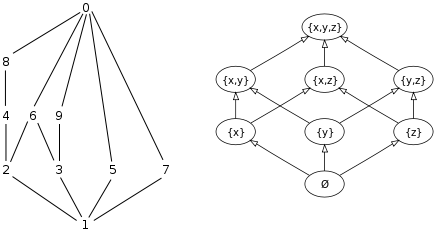
\includegraphics[width=0.7\linewidth]{img/hasse-diagrams.png}
\end{figure}

\sep

\Thm[Cartesian product of posets] For given posets $(A;\preceq)$ and
$(B;\sqsubseteq)$ the relation $\leq$ is defined on $A\times B$ by
\[
(a_1,b_1) \leq (a_2,b_2) :\Longleftrightarrow a_1 \preceq a_2 \land b_1
\sqsubseteq b_2 \]
is a partial order relation. 

\Thm[Lexicographic Order] For given posets $(A;\preceq)$ and $(B;\sqsubseteq)$,
the relation $\leq_{\text{lex}}$ defined on $A\times B$ by
\[
(a_1,b_1) \leq_{\text{lex}}(a_2,b_2) :\Longleftrightarrow a_1 \prec a_2 \lor
(a_1=a_2 \land b_1 \sqsubseteq b_2) \]
is a partial order relation. 

\Lem If both $(A;\preceq)$ and $(B;\sqsubseteq)$ are totally ordered, then so is
the lexicographic order $A\times B$, e.g. $(A\times B;\leq_\text{lex})$.

\sep

\Def[Special Elements] Let $(A;\preceq)$ be a poset, and let $S\subseteq A$ be
some subset of $A$. Then
\begin{enumerate}
  \item $a\in S$ is \textbf{a} \emph{minimal (maximal) element} of $S$ if there
  exists no $b\in S$ with $b\prec a$ $(b\succ a)$.
  \item $a \in S$ is \textbf{the} \emph{least (greatest) element} of $S$ if $a
  \preceq b$ $(a\succeq b)$ for all $b\in S$.
  \item $a\in A$ is \textbf{a} \emph{lower (upper) bound} of $S$ if $a\preceq
  b$ $(a\succeq b)$ for all $b\in S$.
  \item $a \in A$ is \textbf{the} \emph{greatest lower bound $\glb (S)$ (least
  upper bound $\lub (S)$)} of $S$ if $a$ is the greatest (least) element of the
  set of all lower (upper) bounds of $S$.
\end{enumerate}

% TODO: useful comment
\begin{comment}
\Com Note that for a poset $(A;\preceq)$ and a subset $S\subseteq A$,
restricting $\preceq$ to $S$ results in a poset $(S;\preceq)$. Therefore it
would suffice to define minimal and maximal elements for posets rather than
(more generally) for subsets of a poset.

\Com Note also that there can be at most one least element, as suggested by the
word ``the'' in the definition. This follows directly from the antisymmetry of
$\preceq$. If there were two least elements, they would be mutually comparable,
and hence must be equal.

\Com Moreover, note that the definition of the least element and of a lower
bound differ only in that a lower bound can be outside of the considered subset
$S$ (and therefore need not be unique).
\end{comment}

\sep

\Def[Meet and Join] Let $(A;\preceq)$ be a poset. If $a$ and $b$ (i.e., the set
$\{a,b\}\subseteq A$) have a greatest lower bound, then it is called the
\emph{meet} of $a$ and $b$, often denoted $a \land b$. If $a$ and $b$ have a
least upper bound, then it is called the \emph{join} of $a$ and $b$, often
denoted $a \lor b$.

\sep

\Def[Lattice] A poset $(A;\preceq)$ in which every pair of elements has a meet
and a join is called a \emph{lattice}. 

% TODO: useful comment
\begin{comment}
\Ex The poset $(\{0,1,2,3,4,5,6,7,8,9\};|)$ shown in the Hesse-Diagram examples
is a lattice.

\Ex The poset $(\{1,2,3,4,6,8,12,24\};|)$ is also a lattice. The meet of two
elements is their greatest common divisor, and their join is the least common
multiple.
\end{comment}

% TODO: useful comment
\begin{comment}
\sep

\textbf{Examples of Relations}

\begin{tabular}{c|ccc}
& ref. & symm. & trans.\\
\hline
$<\circ |$ 				& 0 & 0 & 0\\
$|\cup \equiv_2$ 		& 1 & 0 & 0\\
$\overline{\equiv_2}$ 	& 0 & 1 & 0\\
$|\cup |^{-1}$ 			& 1 & 1 & 0\\
$ <^2 $ 				& 0 & 0 & 1\\
$ |^{-1}$ 				& 1 & 0 & 1\\
$ <\cap \overline{<}$ 	& 0 & 1 & 1\\
$ \id $ 				& 1 & 1 & 1\\
\end{tabular}
\end{comment}


\subsection{Functions}

\Def[Function] A function $f\colon A \to B$ from a \emph{domain} $A$ to a
\emph{codomain} $B$ is a relation from $A$ to $B$ with special properties (using
the relation notation $a \relf b$):
\begin{enumerate}
  \item $\forall a \in A \ \exists b\in B : a\relf b$ \\($f$ is
  totally defined, ``all $x$-es are assigned''),
  \item $\forall a \in A \ \forall b,b' \in B : a \relf b \land a \relf b' \to
  b=b'$ \\ ($f$ is well-defined, ``unique assignment for each $x$'').
\end{enumerate}

\Def[Set of all Functions] from $A\to B$ is denoted as $B^{A}$.

\Def[Partial Function] is a relation on $A\times B$ such that condition 2. above
holds.

\sep

\Def[Function Equality] Two (partial) functions with common domain $A$ and
codomain $B$ are \emph{equal} if they are equal as relations (i.e., as sets).

\Com $f=g$ is equivalent to saying that the function values of $f$ and $g$ agree
for all arguments (including, in case of partial functions, whether or not it
is defined).

\sep

\Def[Image of a Set] For a function $f:A\to B$ and a subset $S$ of $A$, the
\emph{image} of $S$ under $f$, denoted $f(S)$, is the set
\[
f(S):= \{f(a)|a\in S\}.
\]

\Def[Image] The subset $f(A)$ of $B$ is called the \emph{image} (or
\emph{range}) of $f$ and is also denoted $\im (f)$.

\Def[Preimage of a Set] For a subset $T$ of $B$, the \emph{inverse image} (or
\emph{preimage}) of $T$, denoted $f^{-1}(T)$, is the set of values in $A$ that
map into $T$:
\[
f^{-1}(T):=\{a\in A | f(a) \in T\}.
\]

\sep

\Def[Function Properties] A function $f\colon A\to B$ is called
\begin{enumerate}
  \item \emph{injective} if $\forall a,b\in A \colon \ a\neq b \rightarrow
  f(a)\neq f(b)$
  \item \emph{surjective} if $\forall b \in B \ \exists a \in A \colon \ f(a) =
  b$
  \item \emph{bijective} if it is both injective and surjective.
\end{enumerate}

\sep

\Def[Inverse Function] For a bijective function $f$, the inverse (as a relation
see Definition 3.12) is also a function and is called the inverse function of $f$,
usually denoted as $f^{-1}$.

\sep

\Def[Composition] The \emph{composition} of a function $f\colon A \to B$ and a
function $g\colon B \to C$, denoted by $g\circ f$ or simply $gf$, is defined by
$(g \circ f)(a)=g(f(a))$.

\Lem Function composition is associative (since it's a relation)
\[
(h\circ g)\circ f = h\circ (g \circ f).
\]


\section{Combinatorics and Counting}

\emph{Enumeration} of a set means \emph{listing the lements in a systematic
manner}, and \emph{counting} means \emph{computing the cardinality} of a set.

\subsection{Basic Counting Principles}

\textbf{Addition Principle:} The cardinality of the union of $n$ disjoint finite
sets $A_1, \ldots, A_n$ is equal to the sum of the cardinalities. $\forall
i,j,1\leq i < j \leq n$:
\[
A_i \cap A_j = \emptyset \Longrightarrow |A_1\cup \cdots \cup
A_n|=\sum_{i=1}^{n}|A_i|.
\]

\sep

\textbf{Multiplication Principle:} It is an obvious fact that $|A\times B| =
|A|\cdot |B|$ and more generally, or finite sets $A_1,\ldots,A_n$ the following
holds:
\[
|A_1 \times \cdots \times A_n| = \prod_{i=1}^{n} |A_i|.
\]

\sep

\textbf{Bijection Principle:} If there is a bijection (or one-to-one
correspondence) between the finite sets $A$ and $B$, then $|A|=|B|$.

% TODO: useful comment
\begin{comment}
\Ex The subsets of a finite set $A=\{a_1,\ldots,a_k\}$ with $|A|=k$ are in
one-to-one correspondence with the elements of $\{0,1\}^{k}$, the set of
bit-strings of length $k$. A subset $B\subseteq A$ corresponds to the string
whoes $i$th bit is $1$ if and only if $a_i\in B$. Therefore we have
$|\cP(A)|=2^k$.

\Ex The number of functions $f\colon A \to B$ is $|B|^{|A|}$, since every
function correspons to an element from $B\times B\times \ldots \times B$ (with
$|A|$ factors), the function table of $f$, and vice versa, which means there is
a bijection from the set of functions to the set of $|A|$-tuples over $B$.
\end{comment}

\sep

\textbf{Inclusion-Exclusion Principle:} Is a generalisation of the addition
principle, when two or more sets are not (necessarily) disjoint.

For any finite sets $A_1,\ldots,A_n$,
\begin{align*}
|A_1\cup\cdots\cup A_n| = &\sum_{i=1}^{n}|A_i|
- \sum_{\mathclap{1\leq i_1 < i_2 \leq n}}|A_{i_{1}} \cap A_{i_{2}}|
+ \sum_{\mathclap{1\leq i_1 < i_2 < i_3\leq n}}|A_{i_{1}} \cap A_{i_{2}}
\cap A_{i_{3}}|
\\
&- \ldots +(-1)^{n-1}|A_{1} \cap \cdots \cap A_{n}|\\
\end{align*}

% TODO: useful comment
\begin{comment}
\Ex Count the numbers $n$ $1\leq n \leq 1000$, where $n$ is not divisible by
$3$, $5$ or $11$:

Let
$S:=\{n\in N| 1\leq n \leq 1000\} \rightarrow \card{S}= 1000$

$A_3 := \{n\in S| \ n|3\}$

$A_5 := \{n\in S| \ n|5\}$

$A_{11} := \{n\in S| \ n|11\}$

Hence, we need to determine:
\[
\card{S}-\card{A_3 \cup A_5 \cup A_{11}}.
\]
Where
\begin{align*}
\card{A_3 \cup A_5 \cup A_{11}}
= &\card{A_3} + \card{A_5} + \card{A_11}\\
& - \card{A_3 \cap A_5} - \card{A_3 \cap A_{11}} - \card{A_5 \cap A_{11}}\\
& + \card{A_3 \cap A_5 \cap A_{11}}.
\end{align*}

Lets compute the cardinalities of each component:

$\card{A_3}=\floor{\tfrac{1000}{3}}=333 \ \ (+)$

$\card{A_5}=\floor{\tfrac{1000}{5}}=200 \ \ (+)$

$\card{A_{11}}=\floor{\tfrac{1000}{11}}=90 \ \ (+)$

$\card{A_3 \cap A_5}=\floor{\tfrac{1000}{3\cdot 5}}=66 \ \ (-)$

$\card{A_3 \cap A_{11}}=\floor{\tfrac{1000}{3\cdot 11}}=30 \ \ (-)$

$\card{A_5 \cap A_{11}}=\floor{\tfrac{1000}{5\cdot 11}}=18 \ \ (-)$

$\card{A_3\cap A_5 \cap A_{11}}=\floor{\tfrac{1000}{3\cdot 5\cdot 11}}=6 \ \
(+)$

Now lets put them together
\[
\card{A_3 \cup A_5 \cup A_{11}} = 333 + 200 + 90 - 66 - 30 - 18 + 6 = 515.
\]
Now we have the cardinality of the numbers that are divisible
by $3$, $5$ or $11$. Lets compute the opposite to get the desired result
\[
\card{S}-\card{A_3 \cup A_5 \cup
A_{11}}= 1000 - 515 = \underline{\underline{485}}.
\]

\Com Writing the Fractions in factors (in the floor function) facilitates the
calculation, as we can do the caluclation component wise (divide by the number
that divides 1000, then the ones that yield a remainder).
\end{comment}

\Thm[Bonferroni inequalities] They state that if the
alternating sum in the inclusion-exclusion principle is stopped after counting
the sizes of the unions of $k$ sets, then this is a lower or upper bound for
$|A_1\cup\cdots\cup A_n|$, depending on whether the next sign would be + or
-, respectively, i.e., whether $k$ is even or odd. For instance:
\[
|A_1\cup\cdots\cup A_n| \geq \sum_{i=1}^{n}|A_i|
-\sum_{\mathclap{1\leq i_1 < i_2 \leq n}}|A_{i_{1}}\cap A_{i_{2}}|.
\]

\sep

\Def[Factorial] $k!:=k\cdot(k-1)\cdot(k-2)\cdots 2 \cdot 1$

\Def $n^{\underline{k}}
:=n(n-1)\cdots(n-k+1)=\prod_{i=0}^{k-1}(n-i)=\frac{n!}{(n-k)!}$

\Def[Bin. Coeff.]
$\binom{n}{k}:=\frac{n^{\underline{k}}}{k!}=\frac{n!}{k!(n-k)!}=\frac{n(n-1)
\cdots(n-k+1)}{k!}$\\
$\binom{n}{0}=\binom{n}{n}=1$\\ 
for $k<0$ and $k>n$ we define $\binom{n}{k}:= 0$\\
Can be constructed using Pascal's Triangle with tip $\binom{0}{0}$.\\

\sep

\textbf{Drawing Elements from a Set:} The table shows the umber of possibilities
for selecting $k$ elements from a set of size $n$ (the example set is
$\{a,b,c\}$ thus $n=3$; and $k=2$):

\begin{table}[H]
\resizebox{\columnwidth}{!}{
\begin{tabular}{|l|cc|cc|}
\toprule
 & \multicolumn{2}{c|}{\textbf{Ordered}} &
 \multicolumn{2}{c}{\textbf{Unordered}}\\
 & Number & Examples & Number & Examples\\
\midrule
\shortstack{w.\\ rep.} & $n^k$ &
$\begin{matrix}
aa & ab & ac\\
ba & bb & bc\\
ca & cb & cc
\end{matrix}$
& 
$\binom{n+k-1}{k}$
&
$\begin{matrix}
aa & ab & ac\\
bb & bc &   \\
cc\\
\end{matrix}$\\
\hline
\shortstack{w.o.\\ rep.} &
$n^{\underline{k}}$
&
$\begin{matrix}
ab & ac \\
ba & bc \\
ca & cb\\
\end{matrix}$
&
$\binom{n}{k}$
&
$\begin{matrix}
ab & ac & bc\\
\end{matrix}$\\
\bottomrule
\end{tabular}
}
\end{table}

\sep

\textbf{Double-Counting Principle:} Consider the problem of counting a
subset $S$ of $A\times B$ (wich can also be interpreted as a relation). We can
count $S$ in two different ways, either by determining for each $a\in A$ the
number $m_a$ of $b\in B$ such that $(a,b)\in S$, or by determining for each
$b\in B$ the number $n_b$ of $a\in A$ such that $(a,b)\in S$. Then
\[
|S|=\sum_{a\in A}m_a = \sum_{b\in B}n_b
\]
The easiest way to think about this principle is probably to consider the matrix
representation of $S$ (considered as a relation). Then $m_a$ is the number of
1's in the row for $a$, and $n_b$ is the number of 1's in the column for $b$.

% TODO: useful comment
\begin{comment}
\Com If the same set is counted in two different ways, you get the same answer.

\Ex \todo{Use the example marked in orange (summarised)}.

\Ex We need to choose $k$ from $n$ students for a focus group. One of the $k$
chosen students also needs to be chosen as the presenter. Hence, we have
$\binom{n}{k}$ ways to choose $k$ students out of $n$ as focus group and $k$
ways to choose a presenter from a given focus group. Alternatively, we have $n$
ways to choose a presenter and focus group member, and $\binom{n-1}{k-1}$ ways
to choose the remaining focus group members. Hence, 
\[
k\binom{n}{k} = n\binom{n-1}{k-1}.
\]

\Ex See pascal's identity.
\end{comment}

\sep

\textbf{Pigeonhole Principle: } If a set of $n$ objects is partitioned into
$k<n$ sets, then at least one of these sets contains at least
$\ceil{\tfrac{n}{k}}$ objects.

% TODO: useful comment
\begin{comment}
\Ex If there are $15$ birds and $10$ boxes and every bird goes into a box, then
there there will be at least one box, which contains at least $2=\ceil{15/10}$
birds.

\Ex Among any ten points locaded on a circle with diameter $5$, there exist at
least two at a distance less than $2$ from each other. Proof: Inscribe a regular
$9$-gon, it wil divide the circle into $9$ equal arcs. The length of the side of
this $9$-gon is $\approx1.71$, and this is an upper bound on the distance of any
two points on the arc. From the pigeonhole principle one of the arcs contains at
least two of the points.

\Ex Prove that having 100 whole numbers, one can choose 15 of them so that the
difference of any two is divisible by 7. Proof: For the difference to be a
multiple of 7, the integers must have equal modulo 7 residues ($7|a-b
\Longrightarrow a\equiv_7 b$). Lets try to pick 100 numbers such that it would
not be possible. To avoid having 15 with the same residue, 14 numbers with
different modulo 7 residues can be picked $14 \cdot 7 = 98$ (For every residue
(there are 7) we pick only 14 (such that there are no 15 belonging to the same
residue)). So far we've only picked 98 numbers. Thus two numbers are left over
and have to share a modulo $7$ residue with the other numbers under the
pigeonhole principle.
\end{comment}

\sep

\subsection{Binomial Coefficients}

\Lem[Symmetry of Pascal's
Triangle]
$
\binom{n}{k}=\binom{n}{n-k}
$

% TODO: useful comment
\begin{comment}
Essentially this lemma states that
pascal's triangle is symmetric. Another way to view this is, that the number of ways
 for selecting $k$ from $n$ is the same as the number of ways of
not-selecting $n-k$ from $n$.
\end{comment}

\sep

\Lem[Pascal's Identity] For $n>0$,
$
\binom{n}{k}=\binom{n-1}{k-1}+\binom{n-1}{k}
$

% TODO: useful comment
\begin{comment}
Here's a combinatorial proof: Consider
all $\binom{n}{k}$ subsets of size $k$ of the set $\{1,2,\ldots,n\}$. Of these,
$\binom{n-1}{k-1}$ subsets contain 1, and $\binom{n-1}{k}$ subsets do not
contain 1. Thus in total there are $\binom{n-1}{k-1}+\binom{n-1}{k}$ subsets of
size $k$.
\end{comment}

\sep

\Thm[Binomial Theorem] For any real (or complex) numbers $x$ and
$y$ and for every integer $n\geq 0$,
\[
(x+y)^n=\sum_{k=0}^{n}\binom{n}{k}x^{n-k}y^k.
\]

% TODO: useful comment
\begin{comment}
\Proof If we expand $(x+y)^n$ without collecting equal terms, we obtain $2^n$
terms of the form $x^ky^n-k$ for some $k$, resulting from selecting in each
factor $(x+y)$ either $x$ or $y$. For a specific $k$, the number of terms is
$\binom{n}{k}$, corresponding to the possible ways to select $k$ times a $y$
from the factors $(x+y)$.
\end{comment}

\Cor These equalities follow from the binomial theorem by setting $x=y=1$ as
well as $x=1$ and $y=-1$.
\[
\sum_{k=0}^{n}\binom{n}{k}=2^n \quad \text{and} \quad
\sum_{k=0}^{n}(-1)^k\binom{n}{k}=0.
\]

% TODO: useful comment
\begin{comment}
The first equality can be proven with the proof of above. The second
equality can also be stated as follows: The sum of the coefficients
$\binom{n}{k}$ with even $k$ is equal to the sum of the coefficients
$\binom{n}{k}$ with odd $k$.
\end{comment}

\sep

\Cor[Vandermonde's Identity] Let $k,m,n\geq 0$ be integers with $m+n > 0$.
Then,
$
\binom{m+n}{k}=\sum_{i=0}^{k}\binom{m}{i}\binom{n}{k-i}
$
In particular,
$
\binom{2n}{n} = \sum_{k=0}^{n}\binom{n}{k}^2.
$

\subsection{Countable and Uncountable Sets}

A set that is countable can be \emph{enumerated} (or listed) by a program (even
though this would take an unbounded time), while an uncountable set can, in
principle, not be enumerated.

\sep

\Def[Cardinality, Countability]

\begin{enumerate}[label=(\roman*)]
  \item Two sets $A$ and $B$ \emph{have the same cardinality}, denoted $A\sim
  B$, if there exists a bijection $A\to B$.
  \item \emph{The cardinality of $B$ is at least the cardinality of $A$},
  denoted $A\preceq B$, if $A\sim C$ for some subset $C\subseteq B$.
  \item $B$ \emph{dominates} $A$, denoted $A\prec B$, if $A\preceq B$ and $A
  \nsim B$.
  \item A set $A$ is called \emph{countable} if $A\preceq \mathbb{N}$, and
  \emph{uncountable} otherwise.
\end{enumerate}

Note that $A\preceq B$ is equivalent to the existence of an injective function
$A\to B	$ (namely the bijection $A\to C \subseteq B$).

\sep

\Lem
\begin{enumerate}[label=(\roman*)]
  \item The relation $\sim$ is an equivalence relation.
  \item The relation $\preceq$ is transitive: $A\preceq B \land B\preceq C
  \Longrightarrow A \preceq C.$
  \item $A\subseteq B \Longrightarrow A \preceq B$.
  \item A subset of a countable set is also countable: $A\subseteq B \land B
  \preceq \mathbb{N} \Longrightarrow A\preceq \mathbb{N}$.
  \item $A\preceq B \land B \preceq A \Longrightarrow A \sim B$.
  \item For two sets $A$ and $B$, exactly one of $A\prec B$, $A\sim B$, and
  $B\prec A$ holds.
\end{enumerate}

% TODO: useful comment
\begin{comment}
\Proof
\begin{enumerate}[label=(\roman*)]
  \item The reflexivity of $\sim $ follows from the fact that the identity
  function is a bijection from $A$ to $A$. The symmetry of $\sim$ holds because
  the inverse of a bijection from $A$ to $B$ is a bijection from $B$ to $A$. The
  transitivity of $\sim$ holds because if there is a bijection from $A$ to $B$,
  and one from $B$ to $C$ then there is one from $A$ to $C$.
  \item Analogous to $(i)$, but with injection.
  \item Injection from $A$ to $B$ exists (identity).
  \item Follows from (ii) and (iii).
  \item Is known as the Bernstein-Schr�der theorem. Its proof is involved and
  beyond the scope of this course.
  \item Consequence of (v).
\end{enumerate}


\sep

An interesting question is: What are the equivalence classes of $\sim$, i.e.,
what are all possible cardinalities of sets. For example, is there a cardinality
between finite and countably infinite? The answer is, no there is not. But there
are infinitely many types of infinity.

\end{comment}

\sep

\Thm For finite sets $A$ and $B$, we have $A\relsim B$ if and only if
$|A|=|B|$. A finite set has never the same cardinality as one of its proper
subsets. Somehwat surprisingly, for infinite sets this is possible.

\sep

% TODO: useful comment
\begin{comment}
\Ex Let $O=\{1,3,5\ldots\}$ be the set of odd natural numbers. Of course, $O$ is
countable since the identity function is a (trivial) injection from $O$ to $\N$.
Actually, there is even a \emph{bijection} $f\colon \N\to O$, namely $n\mapsto
2n+1$. Indeed the theorem states a more general fact:
\end{comment}

\Thm A set $A$ is countable if and only if it is finite or if $A\sim \N$
($A$ is countably infinite).

\Com The theorem can be restated as follows: There is no cardinality level
between finite and countably infinite. Or: if $A\prec \N$, then $A$ is finite.

\sep

\Thm The set $\{0,1\}^*:=\{\epsilon, 0, 1, 00, 01, 10, 11, 000, 001,
\ldots\}$ of finite binary sequences is countable.
\\
\Proof Bijection to $\N$.

\sep

\Thm The set $\N\times \N \ (=\N^2)$ of ordered pairs of naural numbers is
countable.
\\
\Proof Diagonalisation argument.

\sep

\Cor The Cartesian product $A\times B$ of two countable sets $A$ and $B$
is countable, i.e., $A\preceq\N \land B\preceq \N \Longrightarrow A\times
B\preceq \N$.

\sep

\Cor The rational numbers $\Q$ are countable.
\\ 
\Proof Diagonalisation argument.

\sep

\Thm Let $A$ and $A_i$ for $i\in \N$ be countable sets.
\begin{enumerate}[label=(\roman*)]
  \item For any $n\in \N$, the set $A^n$ of $n$-tuples over $A$ is countable.
  \item The union $\cup_{i\in \N}A_i$ of a countable list $A_0,A_1,A_2,\ldots$
  of countable sets is countable.
  \item The set $A^*$ of finite sequences over $A$ is countable.
\end{enumerate}

\sep

\Def Let $\{0,1\}^\infty$ denote the set of semi-infinite binary sequences. Note
that semi-infinite means: bounded in one direction (left), unbounded in the
other (right).

\sep

\Thm The set $\{0,1\}^\infty$ is uncountable.

 TODO: useful comment
\begin{comment}
\Proof Technique: Cantor's diagonalization argument. This is a proof by
contradiction, assume that a bijection $f\colon \N \to \{0,1\}$ esists. Let
$\beta_{i,j}$ be the $j$th bit in the $i$-th sequence $f(i)$, where for
convenience we begin numbering the bits with $j=0$. Let $\overline{b}$ be the
complement of a bit $b\in\{0,1\}$. We define a new semi-infinite binary sequence
$\alpha$ as follows:
\[
\alpha :=
\overline{\beta_{0,0}},\overline{\beta_{1,1}},\overline{\beta_{2,2}},
\overline{\beta_{3,3}},\ldots
\]
Obviously, $\alpha\in\{0,1\}^\infty$, but there is no $n\in \N$ such that
$\alpha = f(n)$ since $\alpha$ is constructed so as to disagree in at least one
bit (actually the $n$th bit) with every sequence $f(n)$ for $n\in\N$. This shows
that $f$ cannot be a bijection, which concludes the proof.
\end{comment}

\sep

% TODO: useful comment
\begin{comment}
\Def{4.3} A function $f\colon \N\to\{0,1\}$	is called \emph{computable} if there
is a program that, for every $n\in\N$, when given $n$ as input, outputs $f(n)$.

\sep

\Cor{4.18} There are uncomputable functions $\N\to\{0,1\}$.

\sep
\end{comment}

\Lem If $A$ is uncountable and $A\preceq B$, then $B$ is uncountable,
i.e.,
\[
A\not\preceq \N \land A\preceq B \Longrightarrow B\not\preceq \N.
\]
In particular, if a subset of a set $B$ is uncountable, then so is $B$.

\sep

\Lem If $A$ is uncountable and $B$ is countable, then $A-B$ is
uncountable.

%TODO: useful comment
\begin{comment}
\Proof By contradiction. If $A-B$ were countable, then $A=(A-B)\cup B$ would
also have to be countable according to Theorem 4.16 (ii). This is a
contradiction.
\end{comment}

\sep

\Thm The set $\R$ of real numbers is uncountable.

\sep

\Thm The interval $[0,1)$ of real numbers is uncountable.

% TODO: facultative chapters?

\section{Graph Theory}

\Def[(Simple) Graph] $G=(V,E)$ consists of a finite set $V$ of vertices (Knoten)
and a set $E\subseteq \{\{u,v\}\subseteq V | u \neq v\}$ of edges (Kanten).

An edge $\{u,v\}$ is said to \emph{connect} the vertices $u$ and $v$. Vertices
connected by an edge are also called \emph{adjacent} (or neighbors).

\sep

\Def[Neighborhood] of a vertex $v$ is the set
\[
\Gamma (v) := \{u\in V | \{u,v\} \in E \}
\] 

\sep

\Def[Directed Graph] $G=(V,E)$ consists of a finite set $V$ of
vertices and a set $E \subseteq V \times V$ of (directed) edges. 

\sep

\Def[In- and Out-Degree] The \emph{in-degree} $\deg^{-}(v)$ of a vertex $v$ is
the number of edges entering $v$, and the \emph{out-degree} $\deg^{+}(v)$ of $v$
is the number of edges leaving $v$.

\sep

\Lem[Sum of Degrees] In a directed graph, 
\[
\sum_{v\in V} \deg^{-}(v) = \sum_{v\in V} \deg^{+}(v) = |E|.
\]
In an undirected graph,
\[
\sum_{v\in V} \deg(v) = 2|E|.
\] 

\sep

\Def[Subgraph] A graph $G = (V,E)$ is a \emph{subgraph} of a graph $H=(V',E')$,
sometimes denoted $G\sqsubseteq H$, if $V\subseteq V'$ and $E \subseteq E'$. 

\sep

\Def[Union] of two graphs $G=(V,E)$ and $H=(V',E')$ is the graph $G\cup H:=(V
\cup V', E\cup E')$.

\Def[Complement] $\overline{G}$ of a graph $G=(V,E)$ is the graph
$\overline{G}=(V,\overline{E})$ where $\overline{E}$ consists of all possible
edges that are not in $E$.

\sep

\Def[Bipartite] A graph $G=(V,E)$ is called \emph{bipartite} if $V$ can be split
into two disjoint sets $V_1$ and $V_2$ of vertices $V=V_1 \cup V_2$, such that no
edge connects two vertices in the same subset $V_i$ $(i=1,2)$. 

\sep

\Def[Adjacency Matrix] $A_G=\left[a_{ij}\right]$ of an undirected
graph $G=(V,E)$ with $V=\{v_1,\ldots,v_n\}$ is the binary $n\times n$ matrix
where
\[
a_{ij} = \begin{cases}
1 & \text{if } \{v_i,v_j\} \in E\\
0 & \text{otherwise. }
\end{cases}
\]
For a directed graph, the condition $\{v_i,v_j\}\in E$ must be replaced by
$(v_i,v_j)\in E$. 

\sep

\Def[Graph Isomorphism] Two graphs $G=(V,E)$ and $H=(V',E')$ are
\emph{isomorphic}, denoted $G\cong H$ if there exists a bijection $\pi \colon V
\leftarrow V'$ such that renaming the vertices of $G$ according to $\pi$
resulsts in $H$, i.e., if $\{u,v\}\in E \Longleftrightarrow \{\pi(u),\pi(v)\}\in
E'.$ \\
For directed graphs the definition is similar, except that $\{u,v\}$ and
$\{\pi(u),\pi(v)\}$ must be replaced by $(u,v)$ and $(\pi(u),\pi(v))$,
respectively.

Note that $\cong$ is an equivalence relation on the set of graphs.

\sep

\Trick To check whether two graphs are isomorph: find the vertices of highest
degree and label them, see if a same path is contained, or check if they are
both bipartite, or check if the both have triangles or other shapes.

\sep

\Def[Contained] A graph $G=(V,E)$ is \emph{contained} in a graph $H=(V',E')$,
denoted $G \preceq H$, if there exists a subgraph $K$ of $H$ that is
isomorphic to $G$:
\[
G\preceq H :\Longleftrightarrow \exists K (G\cong K \land K \sqsubseteq H).
\]

Note that $\preceq$ is a partial order relation on the set of graphs.

\sep

\Def[Complete Graph] on $n$ vertices, denoted $K_n$, is a simple graph with $n$
vertices in which any pair of vertices is connected.

\Def[Empty Graph] is the complement of the complete graph (with no edges).

\Def[$(m,n)$-Mesh] is a graph $M_{m,n}$ on $mn$ vertices with
\\
$V=\{(i,j)|1\leq i\leq m, \ 1\leq j\leq n\}$ and 
\\
$E=\{\{(i,j),(i',j')\} \ | \
(i=i'\land \abs{j-j'}=1) \lor (\abs{i-i'}=1\land j=j')\}$.

\Com the concept of a mesh also extends to higher dimensions.

\Def[$d$-Dimensional Hypercube] $Q_d$ is a graph on $V=\{0,1\}^d$
with $\{u,v\}\in E$ if and only if $u$ and $v$ differ in exactly one bit. 

\Def[Complete Bipartite Graph] $K_{m,n}$ is a graph on $m+n$
vertices obtained by taking two vertex subsets $B$ and $W$ (for black and
white) of sizes $m$ and $n$, respectively, and connecting each vertex in $B$
with every vertex in $W$, i.e., $K_{m,n}=(V,E)$ with $V=B \cup W$, $B\cap W =
\emptyset$, $|B|=m$, $|W|=n$, and $E=\{\{u,v\}|u\in B \land v \in W\}$. 

\Lem Here some observations about the special graphs
\[
P_2 \cong K_{2,1} \qquad C_4\cong K_{2,2}\cong Q_2 \cong M_{2,2}
\]
\[
P_m\preceq C_n \text{ when }m<n \qquad P_m\not\preceq C_n \text{ for }m\geq n
\qquad C_{2^d}\preceq Q_d
\]

\subsection{Paths and Cycles}

\Def[Various Paths and Cycles trough Graphs] \\
\emph{walk} [Weg]: any edges or vertices
\begin{itemize}[label=\listarrow]
  \item \emph{tour} [Tour]: if all edges are distinct
  \begin{itemize}[label=\listarrow]
    \item \emph{circuit} [Schleife]: if start and endpoint are the same
  \end{itemize}
  \item \emph{path} [Pfad]: if all vertices are distinct\\
  ($\Longrightarrow$ edges must be distinct $\Longrightarrow$ every path is a
  tour)\\
  A path $P_n$ of length $n$ consists of
  \vspace{-3pt}
  \begin{itemize}[label=$\cdot$,noitemsep,nolistsep,
    topsep=0pt,parsep=0pt,partopsep=0pt]
    \item $n+1$ vertices: $V=\{v_0,\ldots,v_n\}$
    \item $n$ edges: $E=\{\{v_0,v_1\},\{v_1,v_2\},\ldots,\{v_{n-1},v_n\}\}$
  \end{itemize}
  \vspace{-3pt}
  \begin{itemize}[label=\listarrow]
    \item \emph{cycle} [Kreis,Zyklus]: if starting and endpoint are identical\\
    ($\Longrightarrow$ every cycle is a circuit) \\
    A cycle $C_n$ of length $n$ consists of
    \vspace{-3pt}
    \begin{itemize}[label=$\cdot$,noitemsep,nolistsep,
      topsep=0pt,parsep=0pt,partopsep=0pt]
      \item $n$ vertices: $V=\{v_1,\ldots,v_n\}$
      \item $n$ edges: $E=\{\{v_1,v_2\},\ldots,\{v_{n-1},v_{n}\},\{v_n,v_1\}\}$
    \end{itemize}
    \vspace{-3pt}
    \begin{itemize}[label=\listarrow]
      \item \emph{hamiltonian cycle}: if all vertices are visited
    \end{itemize}
  \end{itemize}
\end{itemize}

\sep

\Def[Hamiltionian Graph] a (directed) graph with a \emph{hamiltonian cycle}.

\sep

\Thm In a graph $G$ with adjacency matrix $A_G$ there exists a walk of length
$\ell$ from vertex $u$ to vertex $v$ if and only if the entry at position
$(u,v)$ in $(A_G)^{\ell}$ is not zero. Actually, this entry corresponds to the
number of distinct walks of length $\ell$ from $u$ to $v$.

\sep

\Def[Connected, Components] An undirected graph $G$ is \emph{connected} if any
two vertices are connected by a path. The maximal connected subgraphs of a graph
$G$ are called \emph{components}.

\sep

\Lem The complete graph $K_n$ is trivially hamiltonian. Hence, adding enough
edges will always turn a graph into a Hamiltonian graph.

\Thm A graph $G=(V,E)$ for which 
\[
\card{V}\geq 3
\quad \text{and}\quad
\deg(u)+\deg(v)\geq\card{V}
\]
for every non-adjacent pair $(u,v)$ of vertices
(i.e., $\{u,v\}\not\in E$), is Hamiltionian. In particular
\[
\forall v\in V\colon \deg(v)\geq\frac{\card{V}}{2} \Longrightarrow G \emph { is
Hamiltonian.} \]

\Proof Is done by contradiction assuming a maximal non-Hamiltonian graph
(adding one edge would lead to a Hamiltonian graph), and the conditions of
above. Then one adds the edge, one formalises the hamiltonian cycle. Then by the
pigeonhole principle one can formalise that there would exist another
hamiltonian cycle which contradicts the maximal non-Hamiltonian assumption, and
thus a graph satisfying the conditions must be hamiltonian.

\Thm The hypercube $Q_d$ is Hamiltonian for $d\geq 2$.

\Def{Gray Code} a hamiltonian cycle in a hypercube.

\Lem A bipartite graph can have a Hamiltonian cycle only if the two sets of
vertices have equal size.

\Lem From the previous lemma it follows that the mesh $M_{m,n}$ has no
hamiltonian cycle if both $m$ and $n$ are odd.

\sep

\subsection{Trees}

\Def[Tree] is an undirected connected graph with no cycles. 

\Def[Forest] is an undirected graph with no cycles, i.e., the union of several
trees with disjoint vertex sets . 

\Def[Leaf] is a vertex with degree 1. 

\sep

\Lem A \emph{tree} with $n\geq 2$ vertices has at least 2 leaves. 

\sep

\Thm[Tree Properties] For a graph $G$ with $n$ vertices, the following
statements are equivalent:
\begin{enumerate}[label=(\alph*)]
  \item $G$ is a tree.
  \item $G$ has $n-1$ edges and no cycles.
  \item $G$ has $n-1$ edges and is connected.
\end{enumerate} 

\sep

\Def[Spanning Tree] of a connected graph $G$ is a subgraph of $G$
which is a tree and contains all vertices of $G$. 

\sep

\Def[Rooted Tree] is a tree with a distiguished vertex, the
\emph{root}. There is a unique path from the root to every vertex $v$; its
length is the \emph{distance} of $v$ from the root. The \emph{height}, or
\emph{depth} of the tree is the maximal distance of a leaf from the root. The
vertices on the path from the root to $v$ are called \emph{ancestors} of $v$.
The ancestor which is a neighbor of $v$ is called the \emph{parent}, and $v$ is
called a \emph{child} of the parent. A rooted tree is a \emph{$d$-ary tree} if
every vertex has at most $d$ children. 

\sep

\subsection{Planar Graphs}

Note that graph can always be embedded without crossings in three-dimensional
space.

\sep

\Def[Planarity] A graph is \emph{planar} if it can be drawn in the plane with no
edges crossing. 

\sep

\Def[Regions, Degree] A drawing of a planar graph divides the plane into
disjoint \emph{regions}, one of which is infinite. The \emph{degree} of a region
is the number of edges one encounters in a walk around the region's boundary.
(An edge is counted twice if the edge is a bridge.)

\sep

\Thm[Euler's formula] A plane drawing of a connected planar graph
$G=(V,E)$ divides the plane into $r:=|E|-|V|+2$ regions. 

\Lem For any connected planar graph $G=(V,E)$, the sum of the degrees of
the regions is equal to $2|E|$. 

\Thm Every connected planar graph $G=(V,E)$ with $|V|\geq 3$ satisfies
\[
|E|\leq 3|V| -6.
\]
If $G$ is bipartite, then the following stronger inequality holds:
\[
|E|\leq2|V|-4.
\]
 
\sep

\Cor $K_n \text{ is planar }\Longleftrightarrow \ n\leq 4$. 

\sep

\Cor $K_{3,3}$ is not planar. 

\sep

\textbf{Planarity Preserving Operations}\\
We can define three operations on a graph:
\begin{enumerate}
  \item deletion of edges,
  \item deletion of singleton vertices, and
  \item merging neighboring vertices, i.e., deleting the edge between them,
  replacing the two vertices by a single vertex and maintaining all the edges
  from the two (merged) vertices.
\end{enumerate}

\Lem If a sequence of these three operations is performed on a graph $G$
and the resulting graph $H$ is non-planar, then also $G$ is non-planar. 

% TODO: useful comment
\begin{comment}
\sep

Proof. Each of these operations preserves planarity. Hence if $G$ is planar,
then so must be $H$. Thus if $H$ is non-planar, so must be $G$.
\[
G \text{ planar } \Longrightarrow H \text{ planar }
\]
\[
H \text{ not planar } \Longrightarrow  G \text{ not planar }
\]
\end{comment}

\sep

\Def[Polyhedron] is a solid bounded by a finite number of (plane)
polygon faces. The vertices and edges of these polygons are the vertices and
edges of the polyhedron. A polyhedron is \emph{convex} if the straight line
segment connecting any two points lies entirely within it. A polyhedron is
\emph{regular} if for some $m,n\geq 3$ each vertex meets exactly $m$ faces
(and hence $m$ edges) and each face is a regular $n$-gon. 

\sep

\Thm There are exactly five regular polyhedra, where $(m,n)$ is either
$(3,3),(3,4),(4,3),(3,5), \text{ or }(5,3)$. 

\begin{table}[H]
\resizebox{\columnwidth}{!}{
\begin{tabular}{lcccccc}
\toprule
& $|V|$ & & $|F|$ & $|E|$ & $m=$ Faces met   & $n=$ Edges of\\
&       & & &       & per Vertex & $n$-gons (Faces)\\
\midrule
Tetraeder & 4 & - & 4 & 6 & 3 & 3\\
Hexaeder & 8 & &  6 & 12 & 3 & 4\\
Oktaeder & 6 & \strut\smash{\raise 7pt\hbox{$\times$}} & 8 & 12 & 4 & 3\\
Dodekaeder & 20 & & 12 & 30 & 3 & 5\\
Ikosaeder & 12 & \strut\smash{\raise 7pt\hbox{$\times$}} & 20 & 30 & 5 & 3\\
\bottomrule
\multicolumn{7}{l}{Note that $-$ and $\times$ indicate
the duality.}
\end{tabular}
}
\end{table}



\section{Number Theory}

\subsection{Divisors and Division}

The integers $\mathbb{Z}$ are a special case of a mathematical strucutre called
a \emph{ring}, which will be discussed in Chapter 7. In this chapter we mention
in a few places that concepts like divisors, greatest common divisors, ideals,
etc. can be defined for any ring, not just for the integers.

\sep

\Def[Divisibility] For $a,b\in \Z$ with $a\neq 0$ we define
\[
a|b :\Longleftrightarrow \exists c\in\Z \colon ac=b
\]
($a$=divisor, factor of $b$; $c$=quotient=$\tfrac{b}{2}$; $b$ = mulitple of $a$)

\Com Note that every non-zero integer is a divisor of $0$. Moreover, $1$ and $-1$ are
divisors of every integer.

\Def[Euclid, Quotient Remanider]
\[
\forall a,d\in\Z \ \ (d\neq 0) \ \ \exists! \ q,r\in\Z\colon 
\ a=dq+r \ \land \ 0\leq r \leq \abs{d}
\]
($a$=dividend; $d$=divis.; $q$=quot.; r=remain.=$R_d(a)$=$a\mod d$)

\sep

\Def[A Greatest Common Divisor] $d\neq 0$; $a,b$ not both 0
\begin{align*}
d:=gcd(a,b)
\stackrel{\lnot(a=b=0)}{\Longleftrightarrow} &(d|a\land d|b) \ \land\\
&(\forall c\in \Z-\{0\}\colon c|a\land c|b\Rightarrow
c|d)
\end{align*}

\Def[The Greatest Common Divisor] $=\abs{\gcd(a,b)}$

\Com The concept of a greatest common divisior applies not only to $\Z$, but more
general structures (e.g. polynomial rings). If $d$ and $d'$ are both greatest
common divisors of $a$ and $b$, then $d\mid d'$ and $d'\mid d$. For the integers
$\Z$, this means that $d'=\pm d$, i.e., there are two greatest common divisors.
(But for more general structures there can be more than two greatest common
divisors.)

\Def[Relatively Prime]
\[
a \text{ and } b \text{ are relatively prime }
\Longleftrightarrow
\ gcd(a,b)=1
\]

\sep

\Def[Ideal] generated by $a$ (and $b$)
\[
(a,b) := \{ua+vb \ | \ u,v\in\Z\}
\qquad
(a) := \{ua\ | \ u\in\Z\}
\]

\Lem Every ideal in $\Z$ can be generated by a single integer.
\[
\forall a,b\in \Z \ \text{(not both 0)} \colon (a,b)=(d)\Longrightarrow
d=\pm\gcd(a,b)
\]

\Cor
\[
\forall a,b\in \Z \ \text{(not both 0)} \ \exists u,v\in\Z \colon
\gcd(a,b)=ua+vb
\]

\Thm[Euclid's Extended GCD Algorithm] efficiently computes for given nonnegative
integers $a$ and $b$ with $a\geq b$ (not both 0), the integers $d=\gcd(a,b)$, 
as well as $u$ and $v$ satisfying $ua+vb=\gcd(a,b)$.

Mostly it's used to compute multiplicative inverse mudulo an integer $m$, ie.e
to compute for a given $a$ the integer $b$ such that $R_m(ab)=1$.

\textbf{Application}

How to compute $d:=\gcd(a,b)$ with $a\geq b$ as well as $u$ and $v$ satisfying
$ua+vb=\gcd(a,b)=:d$.


\resizebox{\columnwidth}{!}{
\begin{tabular}{l|c|cc|cc|cc}
& $q$ & $s_1$ & $s_2$ & $u_1$ & $u_2$ & $v_1$ & $v_2$ \\
\hline
after init     & $\lfloor \frac{a}{b} \rfloor$  & $a$ &  $b$ &   1 &    0 &   
0   & 1\\
after n-th loop &  $\lfloor \frac{s_1}{s_2} \rfloor $ & $s_2$ &
$s_1-qs_2=:R_{s_2}(s_1)$ & $u_2$ & $u_1-qu_2$ & $v_2$ & $v_1 - qv_2$\\
term. if    & & $\underline{\underline{s_2}}$ & $\boxed{\leq 0}$ &
$\underline{\underline{u_2}}$ & & $\underline{\underline{v_2}}$
\end{tabular}
}

Then the result is: $d:=s_1, \ u=u_1, \ v=v_1;$

(You can just compute the values of the next line with the values from the
previous line (Except $q$ which is computed from the values of the current
line, and is done last).
Stop calculation the next line if the termination condition was met in the
 previous line.)

\textbf{Example: $\gcd(789,22)$}

\resizebox{\columnwidth}{!}{
\begin{tabular}{l|c|ccc|ccc|ccc}
& $q$ & $s_1$ & & $s_2$ & $u_1$ & & $u_2$ & $v_1$ & & $v_2$ \\
\hline
after init     & 35 & 789 & & 22 &  1 & &   0 &    0 & &    1\\
after 1st loop &  1 &  22 & \strut\smash{\raise
7pt\hbox{$\mathclap{\swarrow}$}}& 19 &  0 &\strut\smash{\raise
7pt\hbox{$\mathclap{\swarrow}$}} & 1 & 1 &\strut\smash{\raise 
7pt\hbox{$\mathclap{\swarrow}$}} &  -35\\
after 2nd loop &  6 &  19 & \strut\smash{\raise
7pt\hbox{$\mathclap{\swarrow}$}}&  3 &  1 &\strut\smash{\raise
7pt\hbox{$\mathclap{\swarrow}$}} &  -1 &  -35 &\strut\smash{\raise 
7pt\hbox{$\mathclap{\swarrow}$}} &   36\\
after 3rd loop &  3 &   3 & \strut\smash{\raise
7pt\hbox{$\mathclap{\swarrow}$}}&  1 & -1 &\strut\smash{\raise
7pt\hbox{$\mathclap{\swarrow}$}} &   7 &   36 &\strut\smash{\raise 
7pt\hbox{$\mathclap{\swarrow}$}} & -251\\
after 4th loop &    &   \underline{\underline{1}} &\strut\smash{\raise
7pt\hbox{$\mathclap{\swarrow}$}} &  \boxed{0} & \underline{\underline{7}}
&\strut\smash{\raise 7pt\hbox{$\mathclap{\swarrow}$}} &  &
\underline{\underline{-251}} & \strut\smash{\raise
7pt\hbox{$\mathclap{\swarrow}$}}
\end{tabular}
}


\subsection{Factorisation into Primes}

\Def[Prime] A positive integer $p>1$ is called \emph{prime} if the only positive
divisors of $p$ are $1$ and $p$.

\Def[Composite]  An integer greater than $1$ that is not a prime
is called \emph{composite}.

\Com This notion of having only trivial divisors extends to other rings, for
example $\R[x]$. In such a general context, the property is called \emph{irreducible}
rather than \emph{prime}. 

The term \emph{prime} is in general used for the
property that if $p$ divides a product of elements, then it divides at least one
of them. 

For the integers, these two concepts are equivalent. The next lemma
states one direction of this equivalence.

\sep

\Lem If $p$ is a prime which divides the product $x_1x_2\cdots x_n$ of some
integers $x_1,\ldots,x_n$, then $p$ divides one of them, i.e. $p\mid x_i$ for
some $i\in\{1,\ldots,n\}$.
\[
p \emph{ is prime } \land p|x_1x_2\cdots x_n \Longrightarrow
\exists i\in\{1,\ldots,n\} \colon p|x_i
\] 

\sep

\Thm[Fundamental Theorem of Arithmetic] Every positive integer can be written
uniquely (up to the order in which factors are listed) as the product of primes. 

\sep

\Thm $\sqrt{n}$ is irrational unless $n$ is a square ($n=c^2,\
\text{for }c\in\Z$).

\sep

\Def[Least Common Multiple] $l$ of two positive integers $a$ and
$b$, denoted $l=\lcm(a,b)$, is the common multiple of $a$ and $b$ which divides
every common multiple of $a$ and $b$, i.e., $a\mid l$, $b\mid l$, $l>0$, and
\[
(l=\lcm(a,b))\qquad 
a\mid l' \land b\mid l' \Longrightarrow l\mid l'.
\] 

\sep

\textbf{Building GCD and LCM of Prime Factorisation of $a$ and $b$}

% TODO: useful comment
\begin{comment}
The least common multiple is in a sense a dual concept of the greatest common
divisor. It is clear from what follows that $\lcm(a,b)$ is well-defined and
unique. The fundamental theorem of arithmetic assures that integers $a$ and $b$
can be written as
\end{comment}
\[
a = \prod_{i} p_i^{e_i} \qquad  \qquad b = \prod_{i} p_i^{f_i}
\]

% TODO: useful comment
\begin{comment}
This product can be understood in two different ways. Either it is over all
primes, where all but finitely many of the $e_i$ are $0$, or it is over a fixed
agreed set of primes. Either view is correct. Now we have
\end{comment}
\[
\gcd (a,b) = \prod_{i} p_i^{\min(e_i,f_i)}
\qquad 
\lcm (a,b) = \prod_{i} p_i^{\max(e_i,f_i)}.
\]
It is easy to see that:
\[
\gcd(a,b) \cdot \lcm(a,b) = ab.
\]

\sep

One can easily derive the following rules from the prime factorisation.
\begin{align*}
even + even &= even  &  even \cdot even &= even \\
even + odd  &= odd   &  even \cdot odd  &= even \\
odd  + odd  &= even  &  odd  \cdot odd  &= odd  \\
\end{align*}

\subsection{Congruences and Modular Arithmetic}

\Def[Congruence] For $a,b,m\in\Z$, $m\geq 1$
\[
a\equiv b\ (\text{mod }  m)
:\Longleftrightarrow
a\equiv_m b
:\Longleftrightarrow
m|(a-b)
\]
``$a$ is congruent to $b$ modulo $m$''

\Lem For any $m\geq 1$, $\equiv_m$ is an equivalence relation on $\Z$.

\Com There are $m$ equivalence classes, namely $[0],[1],\ldots,[m-1]$. Each
equivalence class $[a]$ has a natural representative $R_m(a)\in[a]$ in the set
$\Z_m:={0,1,\ldots,m-1}$ of remainders modulo $m$.

\Lem[Compatibility with Arithmetic Operations]
\[
(a\equiv_m b) \ \land \ (c\equiv_m d) 
\ \Longrightarrow \ 
(a+c\equiv_m b+d) \ \land \ (ac\equiv_m bd)
\]

\Cor Let $f(x_1,\ldots,x_k)$ be a multi-variate polynomial in $k$
variables with integer coefficients, and let $m\geq 1$. If $a_1\equiv_m b_i$
for $1\leq i\leq k$, then $f(a_1,\ldots,a_k)\equiv_m f(b_1,\ldots,b_k)$. 

\sep

\textbf{Good to know:}
If an equality holds over the integers, then it must also hold over any modulus
$m$. In other words,
\[
a=b \Longrightarrow a\equiv_m b
\]
The implication can be turned around and can be used to prove the inequality of
two numbers $a$ and $b$:
\[
a\not\equiv_m b \Longrightarrow a\neq b
\]

\sep

\Lem For any $a,b,m \in \Z$ with $m\geq 1$,
\begin{enumerate}[label=(\roman*)]
  \item $a\equiv_m R_m(a)$.
  \item $a\equiv_m b \Longleftrightarrow R_m(a) = R_m(b)$.
\end{enumerate}

\Lem For any $a,b,m \in \Z$ with $m\geq 1$,
\begin{enumerate}[label=(\roman*)]
  \item $R_m(a+b) = R_m(R_m(a) + R_m(b))$.
  \item $R_m(ab) = R_m(R_m(a)\cdot R_m(b))$.
\end{enumerate} 

\sep

\Lem
$
(\exists x\in\Z_m \colon \ ax \equiv_m 1) 
\ \Longleftrightarrow \ 
\gcd(a,m) = 1
$
\\
The solution $x$ is unique (use Euclid's GCD).

\Def[Multiplicative Inverse] If $\gcd(a,m) = 1$, the unique solution $x\in\Z_m$
to the congruence equation $ax\equiv_m 1 $ is called the \emph{multiplicative
inverse of $a$ modulo $m$}. One also uses the notation $x\equiv_m a^{-1}$ or
$x\equiv_m 1/a$.

\sep

\Thm[Chinese Remainder Theorem, CRT] Let $m_1,m_2,\ldots,m_r$ be pairwise
relatively prime integers and let $M=\prod_{i=1}^{r}m_i$. For every list
$a_1,\ldots,a_r$ with $0\leq a_i < m_i$ for $1\leq i\leq r$, the system of
congruence equations
\begin{align*}
x&\equiv_{m_1} a_1\\
x&\equiv_{m_2} a_2\\
&\ldots\\
x&\equiv_{m_r} a_r
\end{align*}
for $x$ has a unique solution $x$ satisfying $0\leq x < M$.

\sep

\textbf{Application of CRT}
Compute all $M_i=M/m_i$. Now since $\gcd (M_i,m_i)=1$  there exists an
$N_i$ satisfying
\[
M_i N_i \equiv_{m_i} 1.
\]
Determine all $N_i$ by trying (e.g. increasing $i$ from $0$ to $m_i$).
Then determine the solution $x$ by computing
\[
x=R_M \left(\sum_{i=1}^{r}a_iM_iN_i\right).
\]

\subsection{Diffie-Hellman Key-Agreement Protocol}

\textbf{Color Analogy:} It's hard to mix two colors together. However, it's
almost impossible to find out the two colors that were mixed to obtain a color, since
there are many ways to mix a color.
\vspace{5pt}

\textbf{Lock:} A one-way function that is easy to compute in one direction and
hard to compute in the other direction (e.g. discrete logarithm, $a^x\equiv_k
b$).
\vspace{5pt}

\textbf{Steps:} Assuming you're $A$, and you want to establish a shared secret
key with $B$ without meeting him except through the network:

\begin{figure}[H]
 	\centering
  	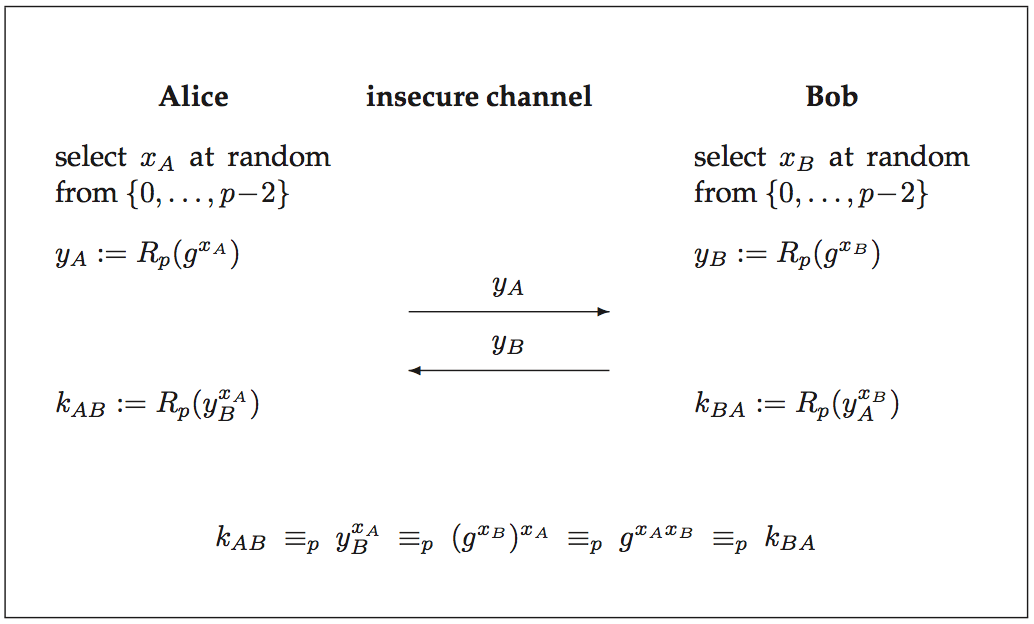
\includegraphics[width=0.9\linewidth]{img/diffie-hellman.png}
\end{figure}

\begin{table}[H]
\resizebox{\columnwidth}{!}{
\begin{tabular}{p{0.035\linewidth}p{0.4\linewidth}p{0.5\linewidth}}
1.) & Agree publicly on a starting color. & Agree publicly on a prime modulus
$p$ and a generator $g$. You may also choose any other finite cyclic group.
\\
2.) & Randomly select a private color (and keep it). & Select your secret $x_A$
from the carrier set.
\\
3.) & Mix the private and public color & Raise the generator $g$ to your secret
$x_A$ to get $y_A$, $y_A=g^{x_A}$.
\\
4.1) & Send the mixture to the other guy $B$. & Send the computed $y_A$ to the
other guy $B$.
\\
4.1) & Receive the color of the other guy $B$. & Receive the computed $y_B$ of
the other guy $B$.
\\
5.) & Add your private color to the received mixture of $B$. This will build the
shared secret color.
& Take the received $y_B$ and raise it to your secret $x_A$. This will yield you
the shared private key $k_{AB}$.
\end{tabular}
}
\end{table}


\section{Logic}

\subsection{Elementary Concepts in Logic}

\begin{comment}
Here, we clearly distinguish between the \emph{syntax} and the \emph{semantics}
of a logic and between \emph{syntactic derivations} of formulas and
\emph{logical consequences} they imply. We also introduce the concept of a
\emph{logical calculus} and define \emph{soundness} and \emph{completeness} of a
calculus.

Examples of useful logics: propositional logic, predicate (or first-order)
logic, temporal logic, modal logic, intuitionistic logic, logics for reasoning
about knowledge and about uncertainit. Most if not all relevant logics contain
the logical operators from propositional logic, i.e., $\land, \lor, \lnot$ (and
the derived operators $\rightarrow$, and $\leftrightarrow$), as well as the
quantifiers ($\forall$ and $\exists$) from predicate logic.

Our goal is to present te general concepts that apply to all types of logics in
a unified manner, and then to discuss the specific instantiations of these
concepts for each logic individually.

\sep
\end{comment}

\Def[Proof System] is a quadruple $\Pi=(\cS,\cP,\tau,\phi)$, where
\begin{description}
\item[$\cS$] is the set of (syntactic representations of) mathematical
statements. Every statement $s\in\cS$ is either true or false.
\item[$\cP$] is the set of proofs. Proofs $p\in\cP$ are also syntactic objects,
for example strings over some alphabet.
\item[$\tau$] The function $\tau\colon\cS\to\{0,1\}$ assigning to each $s\in\cS$
its truth value $\tau(s)$ can be called the \emph{truth function}. This function
defines the meaning, called the \emph{semantics}, of the objects in $\cS$. 
% TODO: useful comment
\begin{comment}
In the context of logic discussed from the next section
onwards, the term semantics is used in a specific manner that is restricted but
compatible in a certain sense with its use here.
\end{comment}
\item[$\phi$] A proof $p$ for a statement $s$ is relative to a
\emph{verification function} $\phi\colon \cS\times\cP \to \{0,1\}$, where
 $\phi(s,p)=1$ means that $p$ is a valid proof for the statement $s$ in the
proof system. Hence, the function $\phi$ defines what is a proof $p\in\cP$ for a
statement $s\in\cS$.
\end{description}

\sep

\Def[Soundness] A proof system $\Pi$ is \emph{sound} (korrekt) if no false
statement has a proof, i.e., if for all $s\in \cS$ for which there exists $p\in
\cP$ with $\phi(s,p)=1$, we have $\tau(s)=1$. This means 
\[ 
\forall s\in \cS \
\forall p\in \cP \colon \quad \phi(s,p)=1 \Longrightarrow \tau(s)=1 
\]

\sep

\Def[Completeness] A proof system $\Pi$ is \emph{complete} if every true
statement has a proof, i.e., if for all $s\in\cS$ with $\tau(s)=1$, there exists
$p\in\cP$, with $\phi(s,p)=1$.

\[
\forall s\in \cS\colon \quad 
\tau(s)=1 \Longrightarrow \exists p\in\cP \ \phi(s,p)=1 
\]

\sep

In addition, one requires that the function $\phi$ is \emph{efficiently
computable} (for some notion of efficiency) and that every true statement has a
reasonably short proof. 

% TODO: useful comment
\begin{comment}
We will not make this formal, but it is obvious that a
proof system is useless if the proof verification is computationally infeasible
or if the shortest proof for a statement with a short description is infeasibly
long.

Also note the following important points:
\begin{itemize}
\item While proof verification must be efficient, \emph{proof generation} is
generally not (or at least not known to be). In general, finding a proof is
generally a process requiring insight and ingenuity, and it cannot e efficiently
automated.
\item A proof system is always restricted (in a sense limited) to a certain type
of mathematical statement. 
\item Proof verification can in principle proceed in very different ways.
\end{itemize}

The goal of logic is to provide a proof system for which a very large class of
mathematical statements can be expressed as an element of $\cS$.

However, such a proof system $\Pi=(\cS,\cP,\tau,\phi)$ can never capture
\emph{all} possible mathematical statements; it usually does not allow to
campture (self-referential) statements about $\Pi$, such as ``$\Pi$ is
complete'', as an element of $\cS$. The use of words i therefore unavoidable in
mathematics.

In logic, the elements of $\cS$ are called formulas, and a proof consists of
applying a certain sequence of syntactic steps, called a \emph{derivation} or a
\emph{deduction}. Each step consists of applying one of  a set of allowed
syntactic rules, and the set of allowed rules is called a \emph{calculus}. A
rule generally has some place-holders that must be instantiated (by some kind
of pattern matching) to perform a step.

In standard treatments of logic, the syntax and sematics of $\cS$ is carefully
defined, but usally the function $\phi$, which consists of verifying the
correctness of each ruel eapplication step, is not explicitly defined. One only
defines rules, but for example one generally does not define a syntax for
expressing how the place-holders of the rules are instantiated. (Of course in a
fully computerized system, this must be defined.)
\end{comment}

\sep

\Def[Syntax] of a logic defines  an alphabet (of allowed symbols) and specifies
which strings (over the alphabet) are syntactically correct formulas.

\sep

\Def[Structure] A formulla generally contains certain variable parts which are
not determined (by the formula) and can take on values in certain domains. A
particular choice of these variable parts is caled a \emph{structure}.

\Def[Suitable Structure] A structure is \emph{suitable} for a formula $F$ if all
variable elements of $F$ are defined (i.e., fixed), i.e., if it makes the
formula true or false. (It may also define \emph{more} variables than the ones
appearing in $F$).

\textbf{Important:} Note that for a structure to be suitable it also needs to
define the \emph{free} variables (i.e., assign them some value!).

\sep

\Def[Semantics] The \emph{sematics} of a logic is a function $\sigma$ assigning
to each formula $F$ and each structure $\cA$ suitable for $F$ a truth value
$\sigma(F,\cA)$ in ${0,1}$.

\sep

\Def[Model] A formula $F$ (or set $M$ of formulas) is called \emph{satisfiable}
if there exists a model $F$ for $M$, and \emph{unsatisfiable} otherwise. The
symbol $\perp$ is used for an unsatisfiable formula.

\sep

\Def[Tautology] A formula $F$ is called a \emph{tautology} or \emph{valid} if it
is true for every suitable structure. The symbol $\top$ is used for a tautology.

\sep

\Def[Logical Consequence] A formula $G$ is a \emph{logical consequence} of a
formula $F$ (or a set $M$ of formulas) denoted $F\models G$ (or $M\models G$),
if every structure suitable for both $F$ (or $M$) and $G$, which is a model for
$F$ (for $M$), is also a model for $G$.

\Def[Equivalence] Two formulas $F$ and $G$ are \emph{equivalent}, denoted
$F\equiv G$ (or also $F\Longleftrightarrow G$), if every structure suitable for
both $F$ and $G$ yields the same truth value for $F$ and $G$, i.e., if each is
logical consequence of the other: $F\equiv G :\Longleftrightarrow	F\models G
\text{ and } G \models F$.

\subsection{Logical Calculi}

\Def[Derivation Rule] is a rule for deriving a formula from a set of formulas
(called the precondition). We write $\{F_1,\ldots,F_k\} \derives_R G$ if $G$ can
be derived from the set $\{F_1,\ldots,F_k\}$ by rule $R$.

\Def[Calculus] A (logical) \emph{calculus} $K$ is a finite set of derivation
rules: $K=\{R_1,\ldots,R_m\}$.

\Def[Derivation] A \emph{derivation of a formula} $G$ from a set $M$ of formulas
in a calculus $K$ is a finite sequence (of some length $n$) of applications of
rules in $K$, leading to $G$.

More precisely, we have $M_0=M$, $M_i:=M_{i-1}\cup\{G_i\}$ for some $R_i\in
K$, and where $G_n = G$. We write $M\derives_K G$ if there is a derivation of
$G$ from $M$ in the calculus $K$.

\Def[Correctness] A derivation rule $R$ is \emph{correct} if for every set $M$
of formulas and every formula $F$
\[
M\derives_R F\Longrightarrow M\models F
\]

\textbf{In other words:} A rule is correct, if it's derivated formula is always
true when it's preconditions are met. As with the implication we need this
``$\leq$'' relation $0\leq 1$ or $0\leq 0$ for all rows.

\sep

\Def[Soundness] A calculus $K$ is \emph{sound} or \emph{correct} if for every
set $M$ of formulas and every formula $F$, if $F$ can be derived from $M$ then
$F$ is also a logical consequence of $M$:
\[
M\derives_K F\Longrightarrow M\models F
\]

\Def[Completeness] A calculus $K$ is \emph{complete} if for every $M$ and $F$,
if $F$ is a logical consequence of $M$, then $F$ can also be derived from $M$:
\[
M\models F\Longrightarrow M\derives_K F
\]

\sep

One writes $\derives_K F$ if $F$ can be derived from the empty set of formulas.

\Lem If $F\derives_K G$ for a sound calculus, then $\models(F\rightarrow G)$.

\sep

\Ex \textbf{A calculus that is not sound} If a calculus has one rule, which is
not correct, like $\{A\lor B\}\derives A \land B$ then the calculus is not
sound (or not correct).

\Ex \textbf{A calculus that is complete, but not sound} The calculus $K:=\{R\}$
with only one rule $\emptyset \derives_R F$. In this calculus, we can derive any
formula from the empty set, however it is not correct. For example deriving
$\emptyset \derives A \land B$ is not correct.

\Ex \textbf{A calculus that is sound, but not complete:}\\
Let $K$ consist of the following two rules.
\[
\{A\land B\} \derives_{R_1} A \qquad \{A,A\rightarrow B\}\derives_{R_2} B
\]
As we can see the Rules $R_1$ and $R_2$ are correct. However, the calculus does
not allow to derive from $B\land A$ the statement $A\land B$, even though
$A\land B\models B\land A$ ($B\land A$ is a logical consequence of $A\land B$).
Hence, there exists a set of formulas, where te calculus does not allow to
derive all its logical consequences from it. Therefore the calculus is not
complete.

\sep

\textbf{Anwendung der Regeln} Beim Anwenden von Regeln muss man immer angeben,
welche Regel man anwendet, welche Formeln man als welches Argument benutzt, und
dann nummeriert man die entstehende Formel (so kann man sie später wieder als
Argument benutzen).

\subsection{Propositional Logic}

\Def[Syntax,Atomic Formula, Formula] An \emph{atomic formula} is of the form
$A_i$ with $i\in \N$. A \emph{formula} is defined inductively: An atomic formula
is a formula, and if $F$ and $G$ are formulas, then also $\lnot F$, $\lnot G$,
$(F\land G)$, and $(F\lor G)$ are formulas.

\sep

\Def[Semantics] For a set $M$ of atomic formulas, a \emph{truth assignment} is a
function $\cA\colon M \to \{0,1\}$. Let $\widehat{M}$ be the set of formulas
built from atomic formulas in $M$. We extend the domain of $\cA$ to
$\widehat{M}$ as follows:
\begin{align*}
\cA((F\land G)) &= 1 \text{ if and only if } \cA(F)=1 \text{ and } \cA(G)=1\\
\cA((F\lor G))  &= 1 \text{ if and only if } \cA(F)=1 \text{ or } \cA(G)=1\\
\cA(\lnot F)  &= 1 \text{ if and only if } \cA(F)=0 
\end{align*}

\sep

\Ex	Extend the propositional logic with the symbol $\oplus$ for the
exlusive or ($A\oplus B$ is exactly then true, when either $A$ or $B$ is true,
but not both). 

\textbf{Syntax:} For all formulas $F$ and $G$, $(F\oplus G)$ is also a formula.

\textbf{Semantics:} $\cA((F\oplus G))=1$ if and only if $\cA(F)=1$ or
$\cA(G)=1$, but not both.

\sep

\textbf{Sprachliche Bedeutung} $A$ kommt nur, wenn auch $B$ kommt. Bedeutet
dasselbe wie $A$ ist nur dann wahr, wenn auch $B$ wahr ist. Das heisst nicht
genau dann wenn. Das heisst mehr ``$A\leq B$''. Das heisst $A\rightarrow B$. 

\sep

\Lem For any formulas $F$, $G$ and $H$ we have
\begin{enumerate}[label=\arabic*)]
  \item $F\land F\equiv  F$ and $F\lor F \equiv F$ (idempotence)
  \item $F\land G\equiv G\land F$ and $F\lor G \equiv G\lor F$ (commutativity)
  \item $(F\land G)\land H \equiv F \land (G\land H)$ and \\$(F\lor G)\lor H
  \equiv F\lor (G\lor H)$ \ \ (associativity)
  \item $F\land(F\lor G)\equiv F$ and $F\lor(F\land G)\equiv F$ (absorption)
  \item $F\land(G\lor H)\equiv (F\land G) \lor (F\land H)$ and\\
  		$F\lor(G\land H)\equiv (F\lor G) \land (F\lor H)$ \ \ (distributive law)
  \item $\lnot \lnot F \equiv F$ (double negation)
  \item $\lnot(F\land G)\equiv \lnot F\lor \lnot G$ and\\
  $\lnot(F\lor G)\equiv \lnot F \land \lnot G$ \ \ (de Morgan's rules)
  \item $F\lor \top\equiv \top$ and $F\land \top \equiv F$ (tautology rules)
  \item $F\lor\perp\equiv F$ and $F\land\perp\equiv \perp$ (unsatisfiability
  rules)
  \item $F\lor\lnot F\equiv \top$ and $F\land \lnot F\equiv \perp$
\end{enumerate}

\sep

\Def[Literal] is an atomic formula or the negation of an antomic formula

\Def[Conjunctive Normal Form (CNF)] A formula $F$ is in CNF if it is a
conjunction of disjunctions of literals, i.e., if it is of the form
$\bigwedge_i \bigvee_j (\neg)x_{ij}$.

The CNF of a Formula can be obtained from its truth table as follows:
For every row where $F=0$, build the disjunction of the inverse of every literal
(i.e., take $\lnot A_i$ if $A_i=1$ and take $A_i$ if $A_i=0$) and then conjunct
the disjunctions.

\Def[Disjunctive Normal Form (DNF)] A formula $F$ is in DNF if it is a
disjunction of conjunction of literals, i.e., if it is of the form
$\bigvee_i\bigwedge_j x_{ij}$.

From a truth table it can be obtained as follows: For every row where $F=1$,
build the conunction of every literal (i.e., take $A_i$ if $A_i=1$, or $\lnot
A_i$ if $A_i=0$) and then disjunct the conunctions.

\Thm Every formula is equivalent to a formula in CNF and also to a formula in
DNF.

\sep

\begin{figure}[H]
 	\centering
  	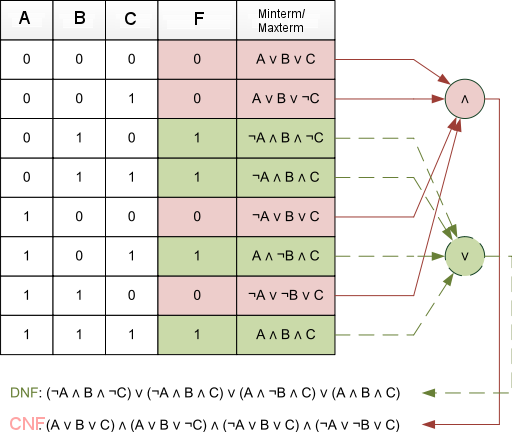
\includegraphics[width=0.87\linewidth]{img/cnf-dnf.png}
\end{figure}

\sep

\Def[Clause] is a set of literals.

\Def[Set of Clauses associated to a Formula] 
\[F=(L_{11}\lor\cdots\lor
L_{1m_1})\land\cdots\land(L_{n1}\lor \cdots\lor L_{nm_n})
\]
in CNF, denoted as $\cK(F)$, is the set 
\[
\cK(F):=\left\{\{L_{11},\ldots,L_{1m_1}\},\ldots,
\{L_{n1},\ldots ,L_{nm_n}\}\right\}
\]
\Def[Set of Clauses Associated with a Set of Formulas] $M=\{F_1,\ldots,F_k\}$
qis the union of their clause sets: $\cK(M):=\cup_{i=1}^k \cK(F_i)$

\Def[Resolvent] A clause $K$ is a \emph{resolvent} of claues $K_1$ and $K_2$ if
there is a literal $L$ such that $L\in K_1$, $\lnot L\in K_2$, and
\[
K=(K_1-\{L\}) \cup (K_2-\{\lnot L\})
\]
Given a set $\cK$ of clauses, a resolution step takes two clauses $K_1\in \cK$
and $K_2\in \cK$, computes a resolvent $K$, and adds $K$ to $\cK$. One can also
write the resolution rule as 
\[
\{K_1,K_2\}\derives_{\text{res}}K,
\]
where the previous equation must be satisfied. The resolution calculus, denoted
Res, consist of a single rule: $Res=\{res\}$.

\Lem The resolution calculus is sound, i.e., if $\cK\derives_{Res}K$ then
$\cK \models K$.

\Thm A set $M$ of formulas is unsatisfiable iff $\cK(M)\derives_{Res}\emptyset$.

\sep

\Ex Show that
\[
G=(\lnot B\land \lnot C \land D)\lor(\lnot B \land \lnot
D)\lor(C\land D)\lor B
\]
is a tautology.

This is true when $\lnot G$ is unsatisfiable. Since $G$ is in DNF we can just
turn it into DNF with de Morgan's rules:
\[
\lnot G=( B\lor C \lor \lnot D)\land( B \lor 
D)\land(\lnot C\lor \lnot D)\land \lnot B
\]
Now, since we have the CNF we can just apply the resolution calculus on the set
of literals to derive the empty set, in order to show that $\lnot G$ is
unsatisfiable. Hence, $G$ is a tautology.

\begin{figure}[H]
 	\centering
  	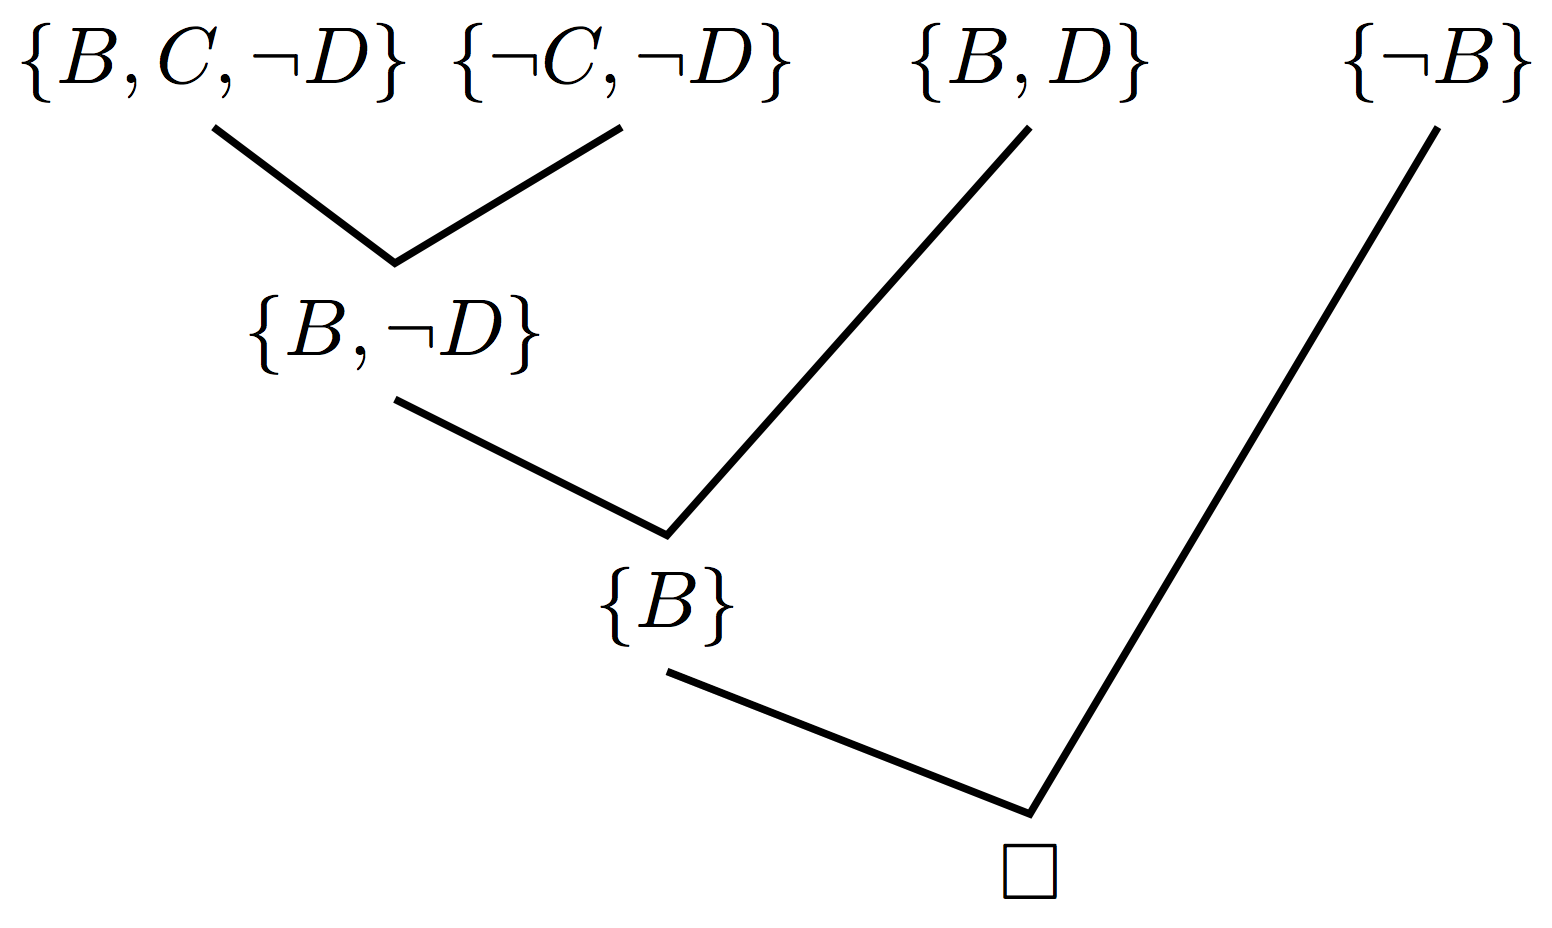
\includegraphics[width=0.55\linewidth]{img/resolution.png}
\end{figure}

\subsection{Predicate Logic}

\Def[Syntax]
\begin{itemize}
  \item A \emph{variable} is of the form $x_i$ with $i\in \N$.
  \item A \emph{function symbol} is of the form $f_i^{(k)}$ with $i,k\in\N$,
  where $k$ denotes the number of arguments of the function. Function symbolds
  for $k=0$ are called \emph{constants}.
  \item A \emph{predicate symbol} is of the form $P_i^{(k)}$ with $i,k\in\N$,
  where $k$ denotes the number of arguments of the predicate.
  \item A \emph{term} is defined inductively: 
  \begin{itemize}
    \item A variable is a term, and if $t_1,\ldots,t_k$ are terms, then
    $P_i^{(k)}(t_1,\ldots,t_k)$ is a formula, called an \emph{atomic} formula.
    \item If $F$ and $G$ are formulas, then also $\lnot F$, $(F\land G)$, and
    $(F\lor G)$ are formulas.
    \item $\forall x_i \ F$ and $\exists x_i \ F$ are also formulas.
  \end{itemize}
\end{itemize}

\sep

\Def[Bounded and Free Variables] Every occurrence of a variable in a formula is
either \emph{bound} or \emph{free}. If a variable $x$ occurs in a (sub-)formula
of the form $\forall x \ G$ or $\exists x \ G$ then it is bound, otherwise it is
free.

\Def[Closed Formula] A formula is \emph{closed} if it contains no free
variables.

\Def[Substitution of Free Variables] For a formula $F$ a variable $x$ and a term
$t$, $F[x/t]$ denotes the formula obtained from $F$ by substituting every free
occurrence of $x$ by $t$.

\sep

\Def[Structure] A \emph{structure} is a tuple $\cA=(U,\phi,\psi,\xi)$ where
\begin{itemize}
  \item $U$ is a \underline{non-empty} set, the so-called \emph{universe},
  \item $\phi$ is a function assigning to each funcition symbol (in a certain
  subset of all function symbols) a function, where for a $k$-ary function
  symbol $f$, $\phi(f)$ is a function $U^k\to{0,1}$, and where
  \item $\xi$ is a function assigning to each variable symbol (in a
  certain subset of all variable symbols) a value in $U$.
\end{itemize}

\sep

\Def[Semantics] For a structure $\cA=(U,\phi,\psi,\xi)$, we define the value
(in $U$) of terms and the truth value of formulas under that structure.
\begin{itemize}
  \item The value $\cA(t)$ of a term $t$ is defined recursively as follows:
  \begin{itemize}
    \item If $t$ is a variable, then $\cA(t)=\xi(t)$.
    \item If $t$ is of the form $f(t_1,\ldots,t_k)$ for some terms
    $t_1,\ldots,t_k$ and a $k$-ary function symbol $f$, then
    \[\cA(t)=\psi(f)(\cA(t_1), \ldots,\cA(t_k)).\]
  \end{itemize}
  \item The truth value of a formula $F$ is defined recursively as follows:
  \begin{itemize}
    \item 
  \end{itemize}
\end{itemize}

\Lem Any equivalence that holds in propositional logic also holds in predicate
logic. Moreover, for any formulas $F$, $G$ and $H$, where $H$ does not contain
the variable $x$, we have
\begin{enumerate}[label=\arabic*)]
  \item $\lnot(\forall x \ F)\equiv \exists x\ \lnot F$
  \item $\lnot(\exists x \ F)\equiv \forall x \ \lnot F$
  \item $(\forall x \ F)\land (\forall x \ G)\equiv \forall x \ (F\land G)$
  \item $(\exists x \ F)\lor (\exists x \ G)\equiv \exists x \ (F\lor G)$
  \item $\forall x \ \forall y \ F \equiv \forall y \ \forall x  \ F$
  \item $\exists x \ \exists y \ F \equiv \exists y \ \exists x  \ F$
  \item $(\forall x \ F)\land H \equiv \forall x \ (F\land H)$
  \item $(\forall x \ F)\lor H \equiv \forall x \ (F\lor H)$
  \item $(\exists x \ F)\land H \equiv \exists x \ (F\land H)$
  \item $(\exists x \ F)\lor H \equiv \exists x \ (F\lor H)$
\end{enumerate}

\sep

\Lem If one replaces a subformula $G$ of a formula $F$ by an equivalent (to $G$)
formula $H$, then the resulting formula is equivalent to $F$.

\sep

\Lem For a formula $G$ in which $x$ occurs only free and in which $y$ does not
occur
\begin{align*}
\forall x \ G &\equiv \forall y \ G[x/y]\\
\exists x \ G &\equiv \exists y \ G[x/y]
\end{align*}

\sep

\Def[Rectified Form] By appropriately renaming quantified variables one can
transform any formula into an equivalent formula in which no variable appears
both as a bound and free variable and such that all variables appearing after
the quantifiers are distinct. Such a formula is said to be in \emph{rectified}
form.

\sep

\Def[Prenex Form] A formula of the form
\[
Q_1x_1Q_2x_2\cdots Q_nx_n \ G
\]
where $Q_i$ are arbitrary quantifiers ($\forall$ or $\exists$) and $G$ is a
formula free of quantifiers, is said to be in \emph{prenex form}.

\sep

\Ex Put $F=\lnot \forall x  \ \exists y \ P(x,y) \land \forall x \ Q(y,x)$ into
prenex form.

Rename $y$ in the right part, since it's a free variable there to avoid name
collisions.
\[
F=\lnot \forall x  \ \exists y \ P(x,y) \land \forall x \ Q(z,x)
\]
Push the $\lnot$ inside on the right side in order to have just quantifiers in
the front.
\[
F=\exists x  \ \forall y \ \lnot P(x,y) \land \forall x \ Q(z,x)
\]
Rename $x$ on the right side in order to avoid name collisions.
\[
F=\exists x  \ \forall y \ \lnot P(x,y) \land \forall a \ Q(z,a)
\]
Move the quantifiers to the front.
\[
F=\exists x  \ \forall y \ \forall a \ \lnot P(x,y) \land Q(z,a)
\]
$F$ is now in prenex form. $z$ is the only free varible $x,y$ and $a$ are bound
variables. It doesn't matter whethere we move $\forall a$ to the front or to the
end of the sequence of quantifiers.


\sep

\Thm The following formula is a tautology:
\[
F:=\lnot \exists x \ \forall y \ (P(y,x)\leftrightarrow\lnot P(y,y))
\]
This means every suitable structure is a model for $F$.

\Proof The formula can be manipulated to say 
\[
\forall x \ \exists y (P(y,x)\leftrightarrow P(y,y) )
\]
which can be always satisfied by choosing $y:=x$.

\Cor There exists no set that contains all sets $S$ that do not contain
themselves, i.e., $\{S|S\not\in S\}$ is not a set.

\Cor The set $\{0,1\}^\infty$ is not countable.

\Cor There are functions $\N\to\{0,1\}$ that are not computed by any program.

\Ex Here we give an example for $\lnot \exists x \ \forall y \
(P(y,x)\leftrightarrow\lnot P(y,y))$

Let 
\begin{itemize}
  \item $U^\cA$ be the set of all men of Zuerich
  \item $P^\cA(x,y)=1$, if $y$ shaves $x$
\end{itemize}

In this case there does not exist a man $x$, such that for all men $y$
(including $x$), $x$ shaves $y$ if and only if $y$ does not shave itself. In the
case of $x$ this would mean ``$x$ shaves $x$ if and only if $x$ does not shave
itself $x$'' which cannot be, therefore no such $x$ exists.

%
\textbf{How to compute modular inverses with gcd}

\todo{How is this done?}

We're looking for the solution $x=a^{-1}$ of
\[
ax\equiv_m=1
\]
Lets transform this, and rename $x$ to $u$ and let $v\in \Z$
\[
au + mv = 1 \Rightarrow au+mv\equiv_m au = 1
\]
Hence if we solve, $\gcd(m,a)$ (since $m>a$) then our solution is $x=u=a^{-1}$.


%%%%%%%%%%%%%%%%%%%%%%%%%%%%%%%%%%%%%%%%%%%%%%%%%%%%%%%%%%%%%%%%%%%%%%%%%%%%%%%%
%%%%%%%%%%%%%%%%%%%%%%%%%%%%%%%%%%%%%%%%%%%%%%%%%%%%%%%%%%%%%%%%%%%%%%%%%%%%%%%%
%%%%%%%%%%%%%%%%%%%%%%%%%%%%%%%%%%%%%%%%%%%%%%%%%%%%%%%%%%%%%%%%%%%%%%%%%%%%%%%%
%%%%%%%%%%%%%%%%%%%%%%%%%%%%%%%%%%%%%%%%%%%%%%%%%%%%%%%%%%%%%%%%%%%%%%%%%%%%%%%%
%%%%%%%%%%%%%%%%%%%%%%%%%%%%%%%%%%%%%%%%%%%%%%%%%%%%%%%%%%%%%%%%%%%%%%%%%%%%%%%%
%%%%%%%%%%%%%%%%%%%%%%%%%%%%%%%%%%%%%%%%%%%%%%%%%%%%%%%%%%%%%%%%%%%%%%%%%%%%%%%%
%%%%%%%%%%%%%%%%%%%%%%%%%%%%%%%%%%%%%%%%%%%%%%%%%%%%%%%%%%%%%%%%%%%%%%%%%%%%%%%%
%%%%%%%%%%%%%%%%%%%%%%%%%%%%%%%%%%%%%%%%%%%%%%%%%%%%%%%%%%%%%%%%%%%%%%%%%%%%%%%%
%%%%%%%%%%%%%%%%%%%%%%%%%%%%%%%%%%%%%%%%%%%%%%%%%%%%%%%%%%%%%%%%%%%%%%%%%%%%%%%%

\section{Algebra Notes}

\Def{*} Let $S_n$ be the set of $n!$ permutations of $n$ elements, i.e., the
set of bijections $\{1,\ldots n\}\to \{1,\ldots,n\}$. The group
$\alg{S_n;\circ,^{-1},\id}$ is called the \emph{symmetric group} of $n$
elements. $S_n$ is non-abelian for $n\geq 3$.

\Com Associativity is a very special property of an operation, but it is of
crucial importance in algebra. Associativity of $*$ means that the element
$a_1*a_2*a_3*\cdots*a_n$ is uniquely defined, independent of the order in which
elements are combined through $*$. This also justifies the use of the notation
$\sum_{i=1}^{n}$ if the operation $*$ is called addition, or $\prod_{i=1}^{n}$
if the operation $*$ is called multiplication.

\textbf{Examples}

\Ex The set of even integers $E$ forms a semigroup (or magma) with respect to
multiplication: $\alg{E;\cdot}$. - There is no neutral element.

\Ex The set uf functions $A\to A$ form a monoid with respect to function
composition: $\alg{A^{A};\circ,\id}$.

\Com To prove the uniqueness of the invers (if it exists), we need $*$ to be
associative:

\Ex Consider again $\alg{A^{A};\circ,\id}$. A function $f\in A^{A}$ has a left
inverse only if it is injective, and it has a right inverse only if it is
surjective. Hence it has only an inverse $f^{-1}$ if and only if $f$ is
bijective. In this case, $f\circ f^{-1} = f^{-1}\circ f = \id$.

\Com We can write $\alg{G;*,\widehat{\ },e}$ instead of $\alg{G;*}$ if we want
to make the inverse operateion an dthe neutral element explicit. Also, often one
simply writes $G$ instead of $\alg{G;*}$ if $*$ is understood. If the operation
$*$ is called addition $(+)$ [multiplication $(\cdot)$], then the inverse of $a$
is denoted $-a$ [$a^{-1}$ or $1/a$] and the neutral element is denoted $0$
[$1$].

\Ex Homomorphism: Projection in $\R^3$ onto a plane and addition.

\Ex Homomorphism: Det. for $n\times n$-Matrices and multiplication.

\Ex The set of symmetries and rotations, denoted $S_\square$, constitutes a
subgroup (with 8 elements) of the set of 24 permutations on $4$ elements.

\Ex The characteristic of $\alg{\Z_m;\oplus,\ominus,0,\cdot,1}$ is $m$. The
characteristic of $\Z$ is 0.

\Ex Set of units of rings: $\Z^*=\{-1,1\}$, $\R^*=\R-\{0\}$ $\C^*=\{1,-1,i,-i\}$.

\Ex Any integer not relatively prime to $m$ is a zerodivisor of $\Z_m$. The set
of units of $\Z_m$ is $\Z^*_m$ (Definition 7.18). A special property of $\Z_m$
is that each non-zero element is either a unit or a zero-divisor.

\Ex $\Z,\Q,\R$, and $\C$ are integral domains.

\Com A polynomial is a formal expression. It can, but need not, be considered as
a function $R\to R$.

\Com The interpretation of ``minus infinity'' is that it is a quantity which
remains unchanged when an arbitrary integer is added to it.

\Ex Fields: $\Q,\R,\C$

\Ex Not Fields: $\Z$ and $R[x]$ for any ring $R$.

\Com Fields are of crucial importance because in a field one can not only add,
subtract, and multiply, but one can also divide by any nonzero element. This is
the abstraction underlying many algorithms like those for solving systems of
linear equations (e.g. by Gaussian elimination) or for polynomial interpolation.
Also, a vector space, a crucial concept in mathematics, is defined over a field,
the so-called base field. Vector spaces over $\R$ are just a special case.


%%%%%%%%%%%%%%%%%%%%%%%%%%%%%%%%%%%%%%%%%%%%%%%%%%%%%%%%%%%%%%%%%%%%%%%%%%%%%%%%
%%%%%%%%%%%%%%%%%%%%%%%%%%%%%%%%%%%%%%%%%%%%%%%%%%%%%%%%%%%%%%%%%%%%%%%%%%%%%%%%
%%%%%%%%%%%%%%%%%%%%%%%%%%%%%%%%%%%%%%%%%%%%%%%%%%%%%%%%%%%%%%%%%%%%%%%%%%%%%%%%
%%%%%%%%%%%%%%%%%%%%%%%%%%%%%%%%%%%%%%%%%%%%%%%%%%%%%%%%%%%%%%%%%%%%%%%%%%%%%%%%
%%%%%%%%%%%%%%%%%%%%%%%%%%%%%%%%%%%%%%%%%%%%%%%%%%%%%%%%%%%%%%%%%%%%%%%%%%%%%%%%
%%%%%%%%%%%%%%%%%%%%%%%%%%%%%%%%%%%%%%%%%%%%%%%%%%%%%%%%%%%%%%%%%%%%%%%%%%%%%%%%
%%%%%%%%%%%%%%%%%%%%%%%%%%%%%%%%%%%%%%%%%%%%%%%%%%%%%%%%%%%%%%%%%%%%%%%%%%%%%%%%
%%%%%%%%%%%%%%%%%%%%%%%%%%%%%%%%%%%%%%%%%%%%%%%%%%%%%%%%%%%%%%%%%%%%%%%%%%%%%%%%
%%%%%%%%%%%%%%%%%%%%%%%%%%%%%%%%%%%%%%%%%%%%%%%%%%%%%%%%%%%%%%%%%%%%%%%%%%%%%%%%


\section{Algebra}

\textbf{General Problem-Solving Approach}
\begin{enumerate}
  \item Eine Seite der zu beweisenden Aussage aufschreiben
  \item Neutrales Element mit Operation an nützlicher Stelle hinzufügen
  \item Neutrales Element geschickt durch anderes bekanntes, das nützlich sein
  könnte ausdrücken
  \item Assoziativität von $*$ oder andere Gruppenaxiome ausnützen
  \item Axiome anwenden, biss gewünschtes auf der rechten Seite steht, q.e.d.
\end{enumerate}

\subsection{Introduction}

\Def[Operation] An \emph{operation} on a set $S$ is a function $S^n\to S$, where
$n\geq 0$ is called the ``\emph{arity}'' of the operation.

% TODO: useful comment
\begin{comment}
\Com Operations with arity $1$ and $2$ are called unary and binary operations,
respectively. An operation with arity 0 is called a constant (or nullary); it is
a fixed element from the set $S$. In many cases, only binary operations are
actually listed explicitly.
\end{comment}

\Def[Algebra] An \emph{algebra} or (\emph{algebraic system} or $\Omega$-algebra)
is a pair $\alg{S;\Omega}$ where $S$ is a set (the \emph{carrier} of the
algebra) and $\Omega=(\omega_1,\ldots,\omega_n)$ is a list of operations on $S$.

% TODO: useful comment
\begin{comment}
There are three levels of abstraction at which one can study algebras.
\begin{itemize}
  \item The \emph{concrete} level: One studies concrete structures and their
  properties.
  \item The \emph{axiomatic} level: One studies a certain class of algebras
  specified by a set of axioms. The axioms are seen as postulates assumed to be
  satisfied for all algebras under consideration. Equivalently, one considers
  all algebras satisfying these axioms, not necessarily with a concrete example
  in mind. Consequences derived from the axioms hold for all algebras in the
  general class of algebras satisfying the axioms.
  \item The \emph{universal} level: One studies algebras without specifying the
  aximos nor the type. For instances, subalgebra, isomorphism, and the direct
  product (see later) are universal algebraic concepts that apply to any
  algebra.
\end{itemize}

Usually, algebra is treated at the abstract axiomatic level, giving examples at
the concrete level. The universal level is considered less frequently.
\end{comment}

\subsection{Semigroups, Monoids, Groups}

(See overview)

\subsection{Homomorphisms and Isomorphisms}

\Def[Homomorphism] A function $\psi$ from a group $\alg{G;*,\widehat{ \ }, e_G}$
to a group $\alg{H;\star,\widetilde{\ }, e_H}$ is a \emph{group homomorphism}
if, for all $a,b\in G$,
\[
\psi(a*b)=\psi(a)\star\psi(b).
\]
\Def[Isomorphism] If $\psi$ is a bijection from $G$ to $H$, then it is called an
\emph{isomorphism}.

\Com Homomorphism $\approx$ structure-preserving function from an algebraic
structure into another algebraic structure

\Lem{7.5} A group homomorphism $\psi$ from $\alg{G;*,\widehat{ \ }, e_G}$ to 
$\alg{H;\star,\widetilde{\ }, e_H}$ satisfies
\begin{enumerate}[label=(\roman*)]
  \item $\psi(e_G) = e_H$,
  \item $\psi(\widehat{a})=\widetilde{\psi(a)}$ for all $a$.
\end{enumerate}




\vspace{100pt}


\subsection*{7.3 The Structure of Groups}

\Def{7.13} A subset $H$ of a group $\alg{G;*,\widehat{ \ }, e}$ is called a
\emph{subgroup} of $G$ if $\alg{H;*,\widehat{ \ }, e}$ is a group, i.e. if $H$
is closed with respect to all operations:
\begin{enumerate}[label=(\arabic*)]
  \item $a*b\in H$ for all $a,b \in H$,
  \item $e\in H$, and
  \item $\widehat{a}\in H$ for all $a \in H$.
\end{enumerate}

\Com For any group $G$ there exist two trivial subgroups: the subset $\{e\}$ and
$G$ itself.

\sep

\todo{In the remainder of this section we will use a multiplicative notation}

\sep

\Def{*} For $n\in \Z$, $a^{n}$ is defined recursively:
\begin{itemize}
  \item $a^0=e$,
  \item $a^n = a\cdot a^{n-1}$ for $n\geq 1$, and
  \item $a^{n} = (a^{-1})^{|n|}$ for $n\leq -1$.	
\end{itemize}

It is easy to see that for all $m,n\in \Z$
\[
a^m\cdot a^n = a^{m+n} \quad \text{and} \quad (a^m)^n = a^{mn}.
\]

\sep

\Def{7.14} Let $G$ be a group and let $a$ be an element of $G$. The \emph{order}
of $a$, denoted $\ord(a)$, is the least $m>1$ such that $a^{m}=e$, if such an
$m$ exists, and $\ord(a)=\infty$ otherwise.

By definition, $\ord(e)=1$.

If $\ord(a)=2$ for some $a$, then $a^{-1}=a$; such
an $a$ is called self-inverse.

\Ex The order of $6$ in $\alg{\Z_{20};\oplus,\ominus,0}$ is $10$. This can be
seen easily since $60=10\cdot 6$ is the least common multiple of $6$ and $20$.
The order of $10$ is $2$, and indeed $10$ is self-inverse.

\sep

\Def{7.15} For a finite group $G$, $\card{G}$ is called the \emph{order} of 
$G$.

\sep

\Lem{7.6} In a finite group $G$, every element has a finite order.

\Proof Since $G$ is finite, we must have $a^{r}=a^{s}=b$ for some $r$ and $s$
with $r<s$ (and some $b$). Then
\[
a^{s-r}=a^s\cdot a^{-r}=a^s\cdot (a^{r})^{-1} = b \cdot b^{-1} = e.
\]

\sep

\Lem{*} If $G$ is a group and $a\in G$ has finite order, then for any $m\in \Z$
we have
\[
a^{m}=a^{R_{\ord(a)}(m)}.
\]

\sep

\Def{7.6} The smallest subgroup of a group $G$ containing the element $a\in G$
is called the \emph{group generated by} $a$, denoted $\alg{a}$, is defined as
\[
\alg{a}:=\{a^n|n\in\Z\}.
\]

\Com For finite groups we have
\[
\alg{a}:=\{e,a,a^2,\ldots,a^{\ord(a)-1}\}.
\]

\sep

\Def{7.17} A group $G=\alg{g}$ generated by an element $g\in G$ is called
\emph{cyclic} and $g$ is called a \emph{generator} of $G$.

\Com Being cyclic is a special property of a group. Not all groups are
cyclic! A cyclic group can have many generators. In particular, if $g$ is a
generator, then so is $g^{-1}$.

\Ex The group $\alg{\Z_n;\oplus}$ is cyclic for every $n$, where $1$ is a
generator. The generators of $\alg{\Z_n,\oplus}$ are all $g\in\Z_n$ for which
$\gcd(g,n)=1$.

\Ex The additive group of the integers, $\alg{\Z;+,-,0}$, is an infinite cyclic
group generated by 1 and also by $(-1)$. These are the only generators. (Note
that negative powers are allowed according to the definition of a group
generated by an element - this allows the reach all the numbers in $\Z$).

\sep

\Thm{7.7} A cyclic group of order $n$ is isomorphic to $\alg{\Z_n;\oplus}$ (and
hence abelian).

\Com In fact, we use $\alg{\Z_n;\oplus}$ as our standard notation of a cyclic
group of order $n$.

\Proof Let $G=\alg{g}$ be a cyclic group of order $n$ (with neutral element
$e$). The bijection
\[
\Z_n\to G\colon i\mapsto g^{i}
\]
is a group isomorphism, since
\[
i\oplus j \mapsto g^{i+j} = g^{i}*g^{j}, \quad
\ominus i \mapsto g^{-i}, \quad
0\mapsto e.
\]

\Com The two groups are $\alg{\Z_n;\oplus;\ominus;0}$ and $\alg{G;*,^{-1},e}$.

\Com It is easy to see that $g^{i}$ is a generator iff $\gcd(i,n)=1$. (Since
$g^{i}\mapsto i \in \Z$, and $i$ is a generator iff $\gcd(i,n)=1$).

\sep

\todo{Integrate the comments about Diffie-Hellman into the according section.}

\sep

The following theorem is one of the fundamental results in group theory, (sated
without proof):

\Thm{7.8} (Lagrange.) Let $G$ be a finite group and let $H$ be a subgroup of
$G$. Then the order of $H$ divides the order of $G$, i.e., $\card{H}$ divides
$\card{G}$.

The following corollaries are direct applications of Lagrange's theorem.

\Cor{7.9} For a finite group $G$ the order of every elements divides the group
order, i.e., $\ord(a)$ divides $\card{G}$ for every $a\in G$.

\Proof $\alg{a}$ is a subgroup of $G$ of order $\ord(a)$, which according to
Theorem 7.8 must divide $\card{G}$.

\Cor{7.10} Let $G$ be a finite group. Then $a^{\card{G}}=e$ for every $a\in G$.

\Proof According to Corollary 7.9 have $\card{G}=k\cdot \ord(a)$ for some $k$.
Hence
\[
a^{\card{G}} = a^{k\cdot \ord(a)} = (a^{\ord(a)})^{k} = e^{k} = e.
\]

\Cor{7.11} Every group of prime order is cyclic, and in such a group every
element, except the neutral element is a generator.

\Proof Let $\card{G}=p$ with $p$ prime. For any $a$, the order of the subgroup
$\alg{a}$ divides $p$. Thus either $\ord(a)=1$ ord $\ord(a)=$. In the first
case, $a=e$ and in the latter case $G=\alg{a}$.

\Com Groups of prime order play a very important role in cryptography.

\sep

\Def{7.18} $\Z^*_m := \{a \in \Z_m | \gcd(a,m) = 1\}$.

\Com $\alg{\Z_m;\odot,^{-1},1}$ must not necessarily be a group, for example in
$\Z_{12}$ 8 has no inverse. Therefore we defined the subset $\Z_{12}^*$. Such
that every element  $\Z_{12}^*$ has an inverse (in contrast to $\Z_{12}$).

\Def{7.19} The \emph{Euler function } $\varphi\colon \Z^+\to\Z^+$ is defined as
the cardinality of $\Z^*_m$:
\[
\varphi(m)=\card{\Z^*_m}.
\]

\Ex $\Z_{18}=\{1,5,7,11,13,17\}.$ Hence $\varphi(18)=6$.

\Lem{7.12} If $m=\prod_{i=1}^{r}p_i^{e_i}$, then
\[
\varphi(m)=\prod_{i=1}^{r}(p_i-1)p_i^{e_i-1}.
\]
Alternatively, $\varphi(m)$ could be defined as
\[
\varphi(m)=m\cdot \prod_{\substack{p|m\\p
\text{ prime}}}\left(1-\frac{1}{p}\right).
\]


\todo{Understand the proof}

\Thm{7.13} $\alg{\Z^*_m;\odot,^{-1},1}$ is a group.

Now we obtain the following simple but powerful corollary to Theorem 7.8:

\Cor{7.14} (Fermat, Euler). For all $m\geq 2$ and all $a$ with $\gcd(a,m)=1$,
\[
a^{\varphi(m)}\equiv_m 1.
\]
In particular, for every prime $p$ and every $a$ not divisible by $p$,
\[
a^{p-1}\equiv_p 1.
\]

\Thm{7.15} The group $\Z^*_m$ is cyclic if and only if $m=2$, $m=4$, $m=p^{e}$,
or $m=2p^e$, where $p$ is an odd prime and $e\geq 1$.

\sep

\todo{Understand pages 119 - 123 including proof and theorems. Finish copying.}

\subsection*{7.4 Rings and Fields}

\todo{don't forget this theorem, it's not on the word document}

\Thm $\Z_p$ is a field if and only if $p$ is prime.

\Proof This follows from our earlier analysis of $\Z^*_p$, namely that
$\Z_p-\{0\}$ is a multiplicative group if and only if $p$ is prime.

\sep

\subsection{Polynomials over Rings and Fields}

Polynomials over a field $F$ are of special interest since they have properties
in common with the integers, $\Z$.

\sep

\Def[Polynomial] $a(x)$ over a ring $R$ or field $F$ in the indeterminate
$x$ is a formal expression of the form
\[
a(x) = a_d x^d + a_{d-1}x^{d-1} + \cdots + a_1x + a_0 = \sum_{i=0}^{d} a_i x^i
\]
for some non-negative integer $d$. The \emph{degree} $\deg(a(x))$ of $a(x)$ is
the greatest $i$ for which $a_i\neq 0$. The special polynomial $0$ (i.e., all
the $a_i$ are 0) is defined to have degree ``minus infinity''. Let $R[x]$ denote
the set of polynomials (in $x$) over $R$.

\sep

\Lem For two polynomials $p(x)$ and $q(x)$ over a ring $R$ the product of two
polynomials is at most the sum of the degrees:
\[
\deg(p(x)\cdot q(x))\leq\deg(p(x)) + \deg(q(x)),
\]
and the equality holds if $R$ is an integral domain
\[
\deg(p(x)\cdot q(x))=\deg(p(x)) + \deg(q(x)),
\]
And in every case, the degree of the sum is:
\[
\deg(p(x)+q(x)) \leq \max\{\deg(p(x)),\deg(q(x))\}.
\]

\sep

\Thm The polynomials over a ring $R$, denoted $R[x]$, are again a ring with
respect to polynomial addition and multiplication.

\sep

\Lem If $D$ is an integral domain, then
  so is $D[x]$. The units of $D[x]$ are the constant polynomials that are units
  of $D$: $D[x]^* = D^*$.

\sep

For $a,b\in \Z$,
\[
b|a \Longleftrightarrow -b|a,
\]
The analogy for polynomials is as follows:
\[
b(x)|a(x) \Longleftrightarrow \forall v\in F, v\neq 0 : v \cdot b(x)|a(x) 
\]
because
\[
a(x)=b(x)\cdot c(x) \Longrightarrow a(x)=v b(x) \cdot \left(v^{-1} c(x)\right).
\]
Among the polynomials $vb(x)$ (for $v\in F$) there is a distinguished one,
namely that with leading coefficient $1$. This is similar to $b$ and $-b$ being
associated in $\Z$ (see section 7.5.3) and the positive one being distinguished.

\sep

\Def[Monic Polynomial] A polynomial $a(x)\in F[x]$ is called \emph{monic} if the
leading coefficient is 1.

\sep

\Def[Irreducible Polynomial] A polynomial $a(x)\in F[x]$ with degree at least
$1$ is called \emph{irreducible} if it is divisible only by constant polynomials
and by constant multiples of $a(x)$.

\Com The notion of irreducibility in $F[x]$	corresponds to the notion of
primality in $\Z$.

\sep

\Lem A polynomial of degree $d$ may be irreducible or reducible. It can be
checked by testing all irreducible polynomials of degree $\leq d/2$ as possible
divisors (but it may also be irreducible).

Actually, it suffices to test only the monic polynomials because one could
always multiply a divisor by a constant. This irreducibility test is very
similar to the primality test which checks all divisors up to the square root of
the number to be tested.

\sep

Not only the concepts of divisors and divison with remainders carres over from
$\Z$ to $F[x]$, also the concept of a greatest common divisor can be carreid
over:

\Def{7.30} For polynomials $a(x)$ and $b(x)$ in $F[x]$ (not both $0$), a
polynomial $d(x)$ is called \emph{a greatest commen divisor} of $a(x)$ and
$b(x)$ if $d(x)|a(x)$ and $d(x)|b(x)$ and if every common divisor of $a(x)$ and
$b(x)$ divides $d(x)$.

Moreover the monic polynomial $g(x)$ of largest degree such that $g(x)|a(x)$ and
$g(x)|b(x)$ is called \emph{the} greatest common divisor of $a(x)$ and $b(x)$,
denoted $\gcd(a(x),b(x))$.

\todo{Algorithm example}

\sep

\subsubsection*{7.5.2 The Division Property in $F[x]$}

Let $F$ be a field. The ring $F[x]$ has strong similarities with the integers
$\Z$. Both these integral domains have the special property that one can divide
one element $a$ by another element $b\neq 0$, resulting in a quiotient $q$ and a
remainder $r$ which are unique when $r$ is required to be ``smaller'' than the
divisor. In case of the integers, the ``soze'' of $b\in \Z$ is given by the
absolute value $\abs{b}$, and the size of a polynomial $b(x)\in F[x]$ can be
defined as its degree $\deg(b(x))$.

\sep

\Thm{7.26} Let $F$ be a field. FOr any $a(x)$ and $b(x)\neq 0$ in $F[x]$ there
exist unique $q(x)$ (the quotient) and $r(x)$ (the remainder) such that
\[
a(x)=b(x)\cdot q(x) + r(x) \quad \text{and} \quad \deg(r(x)) < \deg(b(x))
\]

\sep

\todo{optional section? - have a look.}

\sep

\subsubsection*{7.5.4 Polynomials as Functions}

For a ring $R$, a polynomial $a(x)\in R[x]$ can be interpreted as a function
$R\to R$ by defining \emph{evaluation} of $a(x)$ at $\alpha\in R$ in the usual
manner. This defines a function $R \to R \colon \alpha \mapsto a(\alpha)$.

\sep

\Def{7.34} Let $a(x)\in R[x]$. An element $\alpha \in R$ for which $a(\alpha)=0$
is called a \emph{root} of $a(x)$.

\Lem{7.29} For a field $F$, $\alpha \in F$ is a root of $a(x)$ if and only if
$(x-\alpha)$ divides $a(x)$.

\Lem{*} Lemma 2.29 implies that an irreducible polynomial of degree $\geq 2	$
has no roots.

\Cor{7.30} A polynomial $a(x)$ of degree $2$ or $3$ over a field $F$ is
irreducible if and only if it has no root.

\todo{check proof}

\Def{7.35} If $\alpha$ is a root of $a(x)$, then its \emph{multiplicity} is the
highest power of $(x-\alpha)$ dividing $a(x)$.

\Thm{7.31} For an integral domain (and hence also a field) $D$, a nonzero
polynomial $a(x)\in D[x]$ of degree $d$ has at most $d$ roots, counting
multiplicities.

\todo{check proof}

\subsubsection*{7.5.5 Polynomial Interpolation}

\sep

\Lem[Interpolation Property] A polynomial $a(x)\in F[x]$ of degree at most $d$
is uniquely determined by any $d+1$ values of $a(x)$, i.e., by
$a(\alpha_1),\ldots,a(\alpha_{d+1})$ for any distinct $a_1,\ldots,a_{d+1}\in F$.

\textbf{Lagrange's Interpolation Formula} Let 
\begin{align*}
a(\alpha_1) &= \beta_1\\
a(\alpha_2) &= \beta_2\\
&\vdots\\
a(\alpha_{d+1}) &= \beta_{d+1}
\end{align*}
Then $a(x)$ is given by Lagrange's interpolation formula:
\[
a(x) = \sum_{i=1}^{d+1} \beta_i u_i(x)
\]
where $u_i(x)$ is given by:
\[
u_i(x) = \frac{(x-\alpha_1)\cdots (x-\alpha_{i-1})(x-\alpha_{i+1})\cdots
(x-\alpha_{d+1})}{(\alpha_i -
\alpha_1)\cdots(\alpha_i-\alpha_{i-1})(\alpha_i-\alpha_{i+1})(\alpha_i-\alpha_{d+1})}.
\]

% TODO: useful comment
\begin{comment}
Hence, in $u_i(x)$, the factors, $(x-\alpha_i)$ in the
numerator, and the factor $(\alpha_i-\alpha_i)$ (which would be 0) in the
nominator, are left out.

Note that for $u_i(x)$ to be well-defined, all constant terms $\alpha_i -
\alpha_j$ in the denominator must be invertible. This is guaranteed if $F$ is a
field since $\alpha_i - \alpha_j\neq 0$ for $i\neq j$. Note also that the
denominator is simply a constant and hence $u_i(x)$ is indeed a polynomial of
degree $d$. It eas easy to verify that $u_i(\alpha_i)=1$ and $u_i(\alpha_j)=0$
for $j\neq i$. Thus the polynomials $a(x)$ and $\sum_{i=1}^{d+1}\beta_i u_i(x)$
agree when evaluated at any $\alpha_i$. Note that $a(x)$ has degree at most $d$.

It remains to prove the uniqueness. Suppose there is another polynomial $a'(x)$
of degree at most $d$ such that $\beta_i=a'(\alpha_i)$ for $i=1,\ldots,d+1$.
Then $a(x)-a'(x)$ is also a polynomial of degree at most $d$, which (according
to Theorem 7.31) can have at most $d$ roots, unless it is 0. But $a(x)-a'(x)$
has indeed the $d+1$ roots $\alpha_1,\ldots,\alpha_{d+1}$. Thus it must be 0,
which implies $\alpha(x) = \alpha'(x)$.
\end{comment}

% TODO: useful example
\begin{comment}
\Ex Let $a(x)$ be a polynomial of degree $4$ over $GF(7)[x]$, of which we know
that $a(x)$ has a double root at $x=2$. Further, we know that $a(3)=2$, $a(4)=3$
and $a(6)=5$. Now we want to determine $a(0)$.

First we need to determine $a(x)$. Since $2$ is a double root, $a(x)=(x-2)^2
b(x)$, where $b(x)$ is a polynomial of degree 2.
We know that
\begin{align*}
a(3)=(3-2)^2\cdot b(3)=2 & \Longleftrightarrow b(3)=2 \\
a(4)=(4-2)^2\cdot b(4)=3 & \Longleftrightarrow b(4)= 4^{-1}\cdot 3 = 2 \cdot 3 =6 \\ 
a(6)=(6-2)^2\cdot b(6)=5 & \Longleftrightarrow b(6) = 2^{-1}\cdot 5 = 4
\cdot 5 = 6
\end{align*}
Now we use the Lagrange interpolation to determine $b(x)$:
\begin{align*}
b(x) &= 2 \tfrac{(x-4)(x-6)}{(3-4)(3-6)} + 6 \tfrac{(x-3)(x-6)}{(4-3)(4-6)} +
6\tfrac{(x-3)(x-4)}{(6-3)(6-4)}\\
&= 2 \tfrac{(x-4)(x-6)}{(-1)(-3)} + 6 \tfrac{(x-3)(x-6)}{(-2)} +
6\tfrac{(x-3)(x-4)}{3\cdot 2}\\
&= 2 \tfrac{(x-4)(x-6)}{3} + 6 \tfrac{(x-3)(x-6)}{5} +
6\tfrac{(x-3)(x-4)}{6}\\
&= 2\cdot 3^{-1}(x-4)(x-6)+ 6 \cdot 5^{-1}(x-3)(x-6) +
6 \cdot 6^{-1}(x-3)(x-4)\\
&= 2\cdot 5(x-4)(x-6)+ 6 \cdot 3(x-3)(x-6) + (x-3)(x-4)\\
&= 3(x-4)(x-6)+ 4(x-3)(x-6) + (x-3)(x-4)\\
&= 3(x+3)(x+1)+ 4(x+4)(x+1) + (x+4)(x+3)\\
&= 3(x^2+4x+3)+ 4(x^2+5x+4) + x^2+5\\
&= x^2+4x+2\\
\end{align*}
This gives us:
\begin{align*}
a(x)
&=(x-2)^2 b(x)\\
&=(x+5)^2 (x^2+4x+2)\\
&=(x^2+10x+25) (x^2+4x+2)\\
&=(x^2+3x+4) (x^2+4x+2)\\
&=x^4+7x^3+18x^2+22x+8\\
&=x^4+4x^2+x+1\\
\end{align*}
Therefore $a(0)=1$.
\end{comment}



\subsection{Finite Fields}

So far we have seen the finite field $GF(p)$, where $p$ is prime. In this
section we discuss all remaining finite fields.

\subsubsection*{7.6.1 The Ring $F[x]_{m(x)}$}

We continue to explore the analogies between the rings $\Z$ and $F[x]$. In the
same way as we can compute in the integers $\Z$ modulo an integer $m$, yielding
the ring $\alg{\Z_m;\oplus,\ominus,0,\odot, 1}$, we can also compute in $F[x]$
modulo a polynomial $m(x)$. Let $R_{m(x)}(a(x))$ denote the (unique) remainder
when $a(x)$ is divided by $m(x)$. The concept of congruence modulo $m(x)$ is
defined like congruence modulo $m$. For $a(x),b(x)\in F[x]$,
\[
a(x)\equiv_{m(x)} b(x) :\Longleftrightarrow m(x) | \left(a(x) - b(x)\right).
\]

\sep

\Lem{7.33} Congruence modulo $m(x)$ is an equivalence relation on $F[x]$, and
each equivalence class has a unique representative of degree less than
$\deg(m(x))$.

\Proof Analogous to proof that congruence modulo $m$ is an equivalence relation
on $\Z$.

\sep

\Def{7.36} Let $m(x)$ be a polynomial of degree $d$ over $F$. Then 
\[
F[x]_{m(x)}:=\{a(x)\in F[x] | \deg(a(x)) < d\}.
\]

\sep

\Lem{7.34} Let $F$ be a finite field with $q$ elements and let $m(x)$ be a
polynomial of degree $d$ over $F$. Then $\card{F[x]_{m(x)}}=q^d$.

\sep

\Lem{7.35} $F[x]_{m(x)}$ is a ring with respect to addition and multiplication
modulo $m(x)$.

\Com Note that addition (but not multiplication) in $F[x]$ and $F[x]_{m(x)}$ are
identical, since the sum of two polynomials is never reduced modulo $m(x)$
because the degree of the sum is at most the maximum of the two degrees.

\sep

\Lem{7.36} The congruence equation
\[
a(x)b(x)\equiv_{m(x)}1
\]
(for a given $a(x)$) has a solution $b(x)\in F[x]_{m(x)}$ if and only if
$\gcd(a(x),m(x))=1$. The solution is uniuque - if it exists it is called the
inverse of $a(x)$ modulo $m(x)$. Therefore, we can also define the set of units:
\[
F[x]^*_{m(x)} = \{a(x)\in F[x]_{m(x)} | \gcd(a(x),m(x))=1	\}.
\]

\Com Inverses inf $F[x]^*_{m(x)}$ can be computed efficiently, but we do not
discuss an algorithm here.

\sep

\subsubsection*{7.6.2 Constructing Extension Fields}

The following theorem is analogous to Theorem 7.23 stating that $\Z_m$ is a
field if and only if $m$ is prime.

\Thm{7.37} The ring $F[x]_{m(x)}$ is a field if and only if $m(x)$ is
irreducible.

\Com $F[x]_{m(x)}$ is called an \emph{extension field} of $F$.

\todo{Understand proof!}

\subsection*{7.7 Application: Error-Correcting Codes}









\sep

\textbf{Polynomial Division in a Field}

Here we show how to divide $3x^5 + 9x^2+4x+7$ by $2x^2+x+5$ in $GF(13)$.

First we write the multiplication table with the \emph{coefficients of the
divisor as column titles} and the \emph{elements of $GF(13)$ as rows}: (Don't
forget to think about the spaces if the divisor does not contain all descending powers of $x$.)

\begin{tabular}{c|c|c|c}
   & $x^2$ & $x$ & $c$\\
GF(13)   & 2  &  1 &  5 \\
\hline
 0 &  0 &  0 &  0 \\
 1 &  2 &  1 &  5 \\
 2 &  4 &  2 & 10 \\
 3 &  6 &  3 &  2 \\
 4 &  8 &  4 &  7 \\
 5 & 10 &  5 & 12 \\
 6 & 12 &  6 &  4 \\
 7 &  1 &  7 &  9 \\
 
 \textcolor{green}{8} &  \colorbox{yellow}{\textcolor{red}{3}} & 
 \textcolor{red}{8} &
 \textcolor{red}{1}
 \\
 9 &  5 &  9 &  6 \\
10 &  7 & 10 & 11 \\
11 &  9 & 11 &  3 \\
12 & 11 & 12 &  8 \\
\end{tabular}

Then we write the polynomials divisor and dividend next to each other. It's
important to write the dividend with 0 coefficients for the powers that are not
existing, such that we'll have space to write our steps below.

Now we're ready to execute the polynomial division. We'll always ask us
\emph{what times the leading coefficient of the divisor is equal to the leading
coefficient of the dividend (or the remaining dividend)}. We can find out this
easily as follows, e.g.: 2 times what gives 3? - In the column of the leading
coefficient (in this case 2), wee look where 3 occurs, then we get the
corresponding number at the left of the row: in this case 8 and write it to the
top. Furthermore, copy the contents of the rest of the row for the
subtraction. Then we just do our subtraction in $GF(13)$ until we get the
quotient and the remainder:

\[
\begin{array}{lllllll}
         & \ \ \ \ 8x^3 &+9x^2 & \textcolor{green}{+8}x &+4\\
\cline{2-7}
2x^2+x+5 & | \ \ 3x^5 &+0x^4 &+0x^3 &+9x^2 & +4x & +7\\
         & -3x^5 & -8x^4 & -1x^3\\
\cline{2-4}
         &       & +5x^4 & +12x^3 & +9x^2\\
         &       & -5x^4 & -9x^3  & -6x^2\\
\cline{3-5}
         &       &       & \colorbox{yellow}{+3}x^3  & +3x^2 & +4x\\
         &       &       & \textcolor{red}{-3}x^3  & \textcolor{red}{-8}x^2
         & \textcolor{red}{-1}x\\
\cline{4-6}
         &       &       &        & +8x^2 & +3x & +7\\
         &       &       &        & -8x^2 & -4x & -7\\
\cline{5-7}
         &       &       &        &       & +12x\\
                         
\end{array}
\]

We'll stop with the division as soon as the degree of the remainder is less than
the degree of the divisor.

Finally, the division yields:
\[
q(x) = 8x^3+9x^2+8x+4 \quad \text{(quotient)}
\]
\[
r(x) = 12x \quad \text{(remainder)}
\]

\sep

\textbf{Factoring a Polynomial in a Field}

Lets assume we want to factor the polynomial $x^3+4x+4$ over $GF(7)$. Then we do
the following: Since the degree of the polynomial is $\in\{2,3\}$ we know that
is reducible iff it has a root. Thus we try all numbers in $GF(7)$, e.g.
$\{0,\ldots,6\}$ and take the first matching candidate.

For 4: $4^3+4\cdot 4 + 4 = 2^6 +16 + 4 = 64 + 16 + 4 = 84 \equiv_7 0$.

As we can see $4$ is a root, thus we deflate this root from the polynomial by
dividing with $(x-4)$. The division becomes even easier if we divide by
$(x+3)=(x-4)$, since we're in $GF(7)$.

We'll just divide as described and get.
\[
(x^3+4x+4) : (x+3) = (x^2+4x+6)
\]
Then we get a polynomial of degree 2 : $(x^2+4x+6)$. Trying all the numbers from
0 to 6 shows us that this polynomial of degree 2 is not further reducible. This
gives us the final factorisation:
\[
(x^3+4x+4) = (x+3)(x^2+4x+6).
\]

\sep

\textbf{Irreducible Polynomials over $GF(2)$ of degree $n$:}

\begin{tabular}{lp{.4\textwidth}}
n	& irreducible polynomials\\
1	& $x+1, x$\\
2	& $x^2+x+1$\\
3	& $x^3+x+1$, $x^3+x^2+1$\\
4	& $x^4+x+1$, $x^4+x^3+x^2+x+1$,  $x^4+x^3+1$\\
5   & $x^5+x^2+1$, $x^5+x^3+x^2+x+1$, $x^5+x^3+1$, $x^5+x^4+x^3+x+1$,
$x^5+x^4+x^3+x^2+1$, $x^5+x^4+x^2+x+1$
\end{tabular}

\sep

\textbf{Irreducible Polynomials over $GF(3)$ of degree $n$}:
\begin{tabular}{lp{.4\textwidth}}
n	& irreducible polynomials\\
2	& $x^2 + 2x + 2$, $x^2 + 1$, $x^2 + x + 2$\\
3	& $x^3 + 2x + 1$,
$x^3 + x^2 + x + 2$, 
$x^3 + x^2 + 2$, 
$x^3 + 2x^2 + x + 1$, 
$x^3 + x^2 + 2x + 1$, 
$x^3 + 2x^2 + 2x + 2$, 
$x^3 + 2x + 2$, 
$x^3 + 2x^2 + 1$, 
\end{tabular}

\sep

\textbf{Multiplicative Inverses over Finite Fields}

\begin{tabular}{|c|c|c|c|c|c|c|}
\toprule
& \multicolumn{6}{c|}{$GF(n)$}
\\
          & 2 & 3 & 5 & 7 & 11 &  13\\
\midrule
$1^{-1}$  & 1 & 1 & 1 & 1 &  1 &   1\\
\hline
$2^{-1}$  &   & 2 & 3 & 4 &  6 &   7\\
\hline
$3^{-1}$  &   &   & 2 & 5 &  4 &   9\\
\hline
$4^{-1}$  &   &   & 4 & 2 &  3 &  10\\
\hline
$5^{-1}$  &   &   &   & 3 &  9 &   8\\
\hline
$6^{-1}$  &   &   &   & 6 &  2 &  11\\
\hline
$7^{-1}$  &   &   &   &   &  8 &   2\\
\hline
$8^{-1}$  &   &   &   &   &  7 &   5\\
\hline 
$9^{-1}$  &   &   &   &   &  5 &   3\\
\hline
$10^{-1}$  &   &   &   &   & 10 &  4\\
\hline
$11^{-1}$  &   &   &   &   &    &  6\\
\hline
$12^{-1}$  &   &   &   &   &    & 12\\
\bottomrule
\end{tabular}

\Com $GF(n)$ is isomporph to $\Z_n$. But for the multiplicative group we just
use $\Z_n-\{0\}$ (without $0$, since it has no inverse). Note that in most of
the cases $\Z_n-\{0\}=\Z^*_n$. Further note that there is no field of size
1.

\todo{Note to say what you mean by in most of the cases, if $n$ is prime its
clear. What happens if $n$ is a power of an odd prime? }

\sep

\textbf{Multiplication in $GF(2)[x]_{x^2+x+1}$}

\begin{tabular}{c|cccc}
$\cdot$ & $0$ & $1$ & $x$ & $x+1$\\
\hline
0 & 0 & 0 & 0 & 0\\
1 & 0 & 1 & $x$ & $x+1$\\
$x$ & 0 & $x$ & $x+1$ & 1\\
$x+1$ & 0 & $x+1$ & 1 & $x$
\end{tabular}

\sep

\textbf{Multiplication in $GF(2)[x]_{x^3+x+1}$}

\todo{Table needed?}

\sep

\textbf{Multiplication in $GF(3)[x]_{x^2+1}$}

\todo{Table needed?}


\end{multicols*}

\end{document}